primero de todo descargamos una imagen de debian, para ello vamos a la web de debian https://www.debian.org/distrib/ y elegimos la iso que mejor se adapte a lo que necesitamos, yo en mi caso elegi el instalador a traver de internet
\begin{figure}[H]
    \centering
    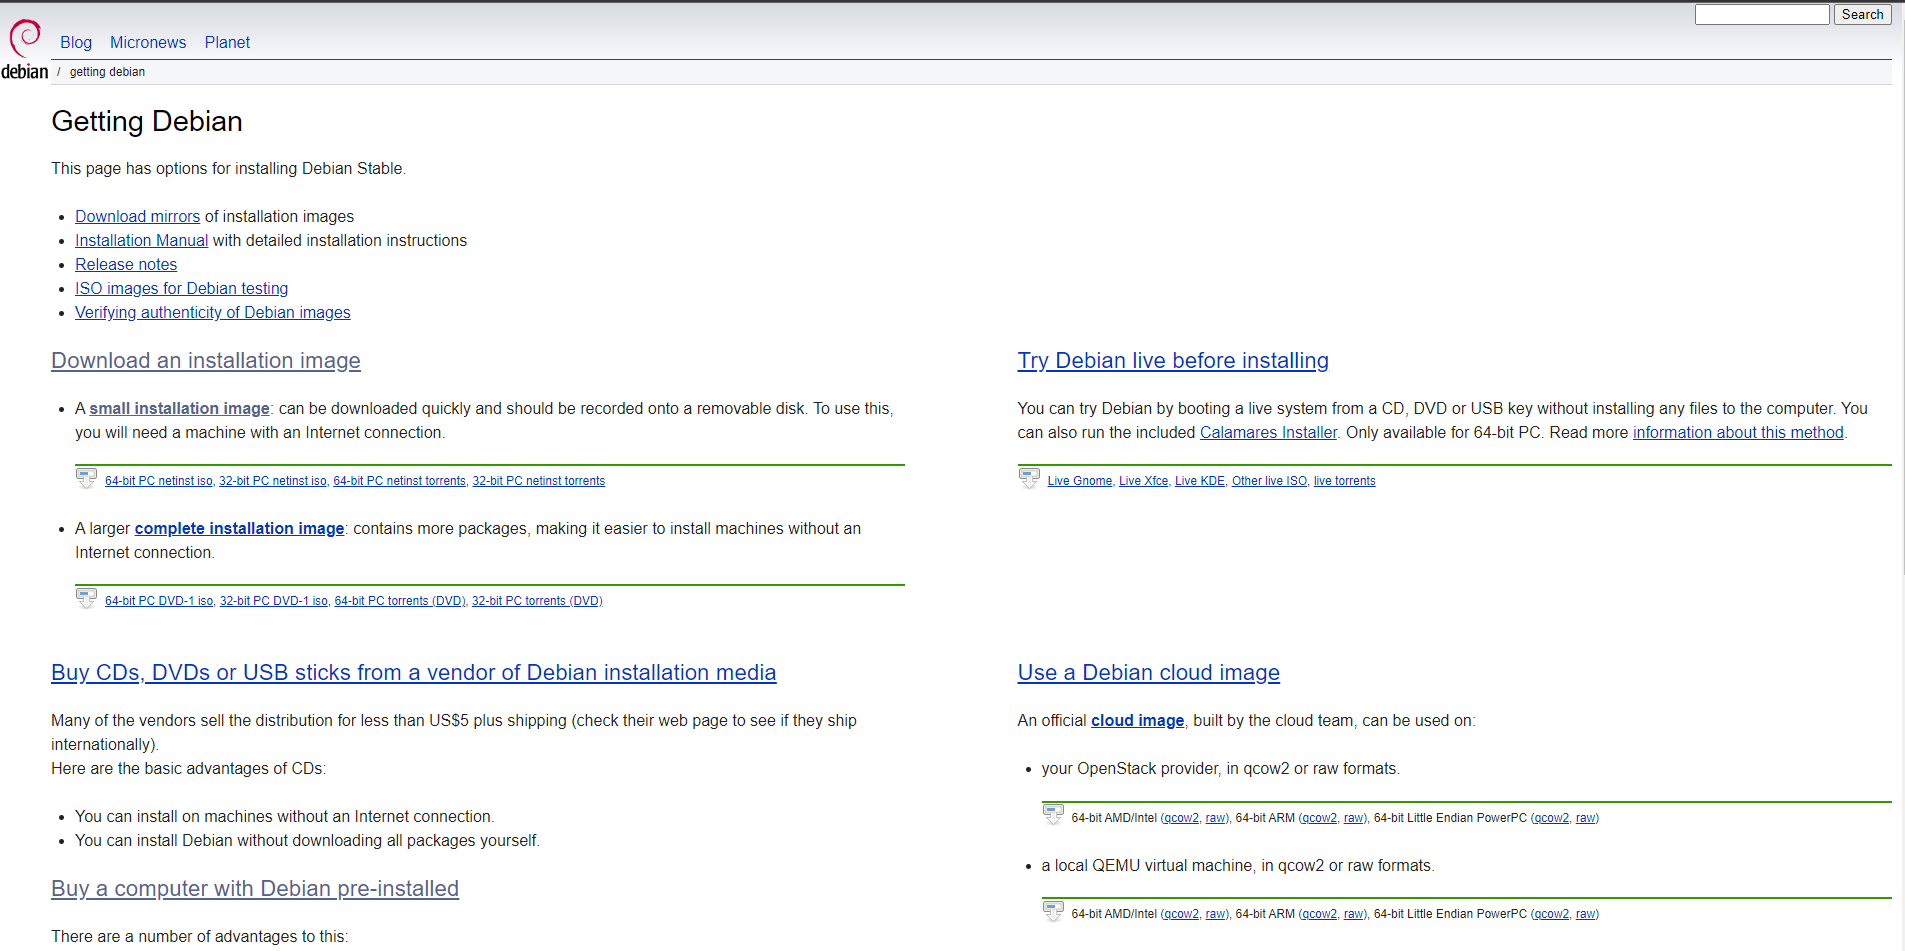
\includegraphics[width=0.5\linewidth]{instalacionBacula/debianPaginaWeb.png}
    \caption{Enter Caption}
\end{figure}
En virtual box añadimos una nueva maquina virtual, le ponemos un nombre y seleccionamos la iso de debian
\begin{figure}[H]
    \centering
    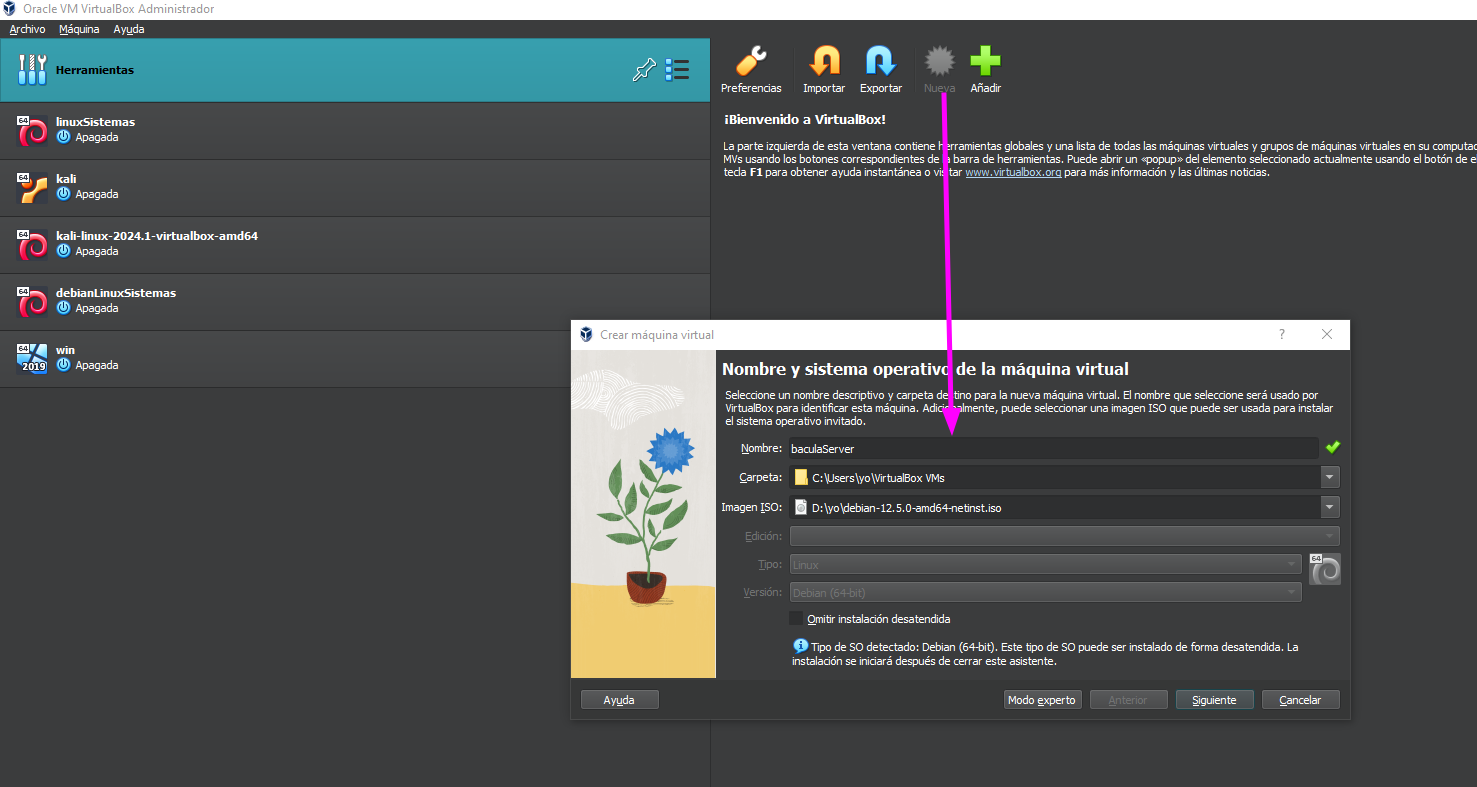
\includegraphics[width=0.5\linewidth]{instalacionBacula/vbDebian.png}
    \caption{Enter Caption}
\end{figure}


Ahora configuramos el usuario y la contranseña de la maquina:

\begin{figure}[H]
    \centering
    \includegraphics[width=0.5\linewidth]{instalacionBacula/instalación desatendida del SO.png}
    \caption{Enter Caption}
\end{figure}

Configuramos el hardware, debian no es un sistema operativo muy pesado y no necesita muchos recursos para que funcione de forma fluida, asique no es necesario darle mucha memoria base y procesadores:
\begin{figure}[H]
    \centering
    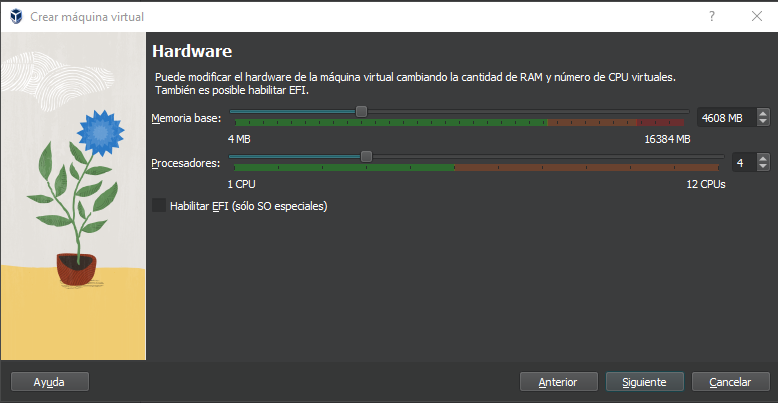
\includegraphics[width=0.5\linewidth]{instalacionBacula/vbhardware.png}
    \caption{Enter Caption}
\end{figure}

Ahora necesitamos asignarle el almacenamiento para ello creamos un disco duro virtual, y le asignamos 50 GB
\begin{figure}[H]
    \centering
    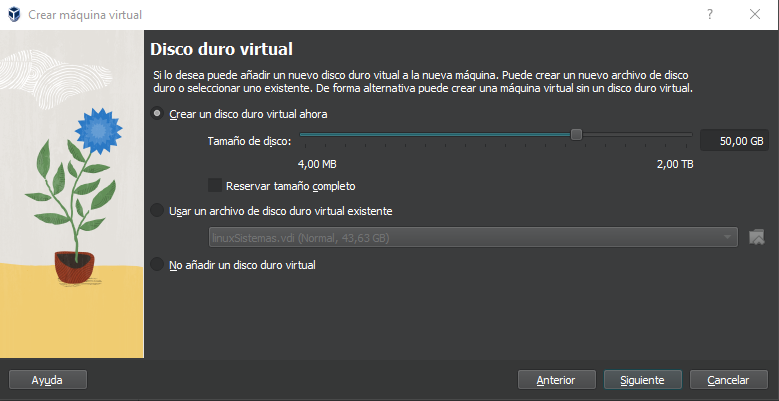
\includegraphics[width=0.5\linewidth]{instalacionBacula/vbDisco.png}
    \caption{Enter Caption}
\end{figure}

Ahora instalamos y dejamos que el instalador haga su trabajo.

Una vez instalado realizamos en la consola un upgrade y un update del sistema:

\begin{figure}[H]
    \centering
    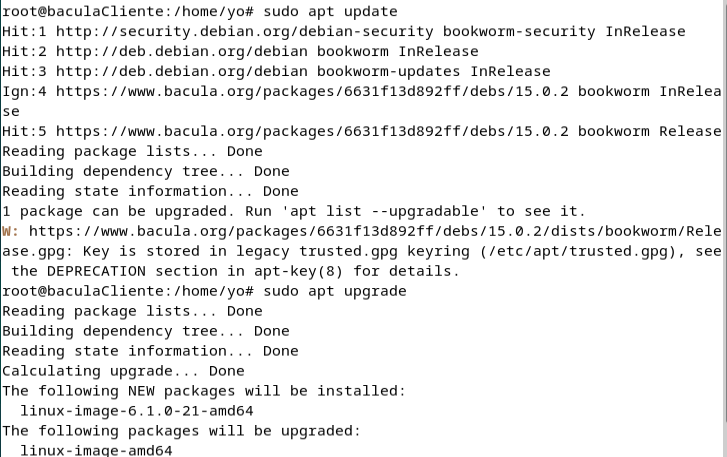
\includegraphics[width=0.5\linewidth]{instalacionBacula/Update y upgrade.png}
    \caption{Enter Caption}
\end{figure}

Finalmente en la configuracion en virtual box cambiamos la red de nat a adaptador puente:

\begin{figure}[H]
    \centering
    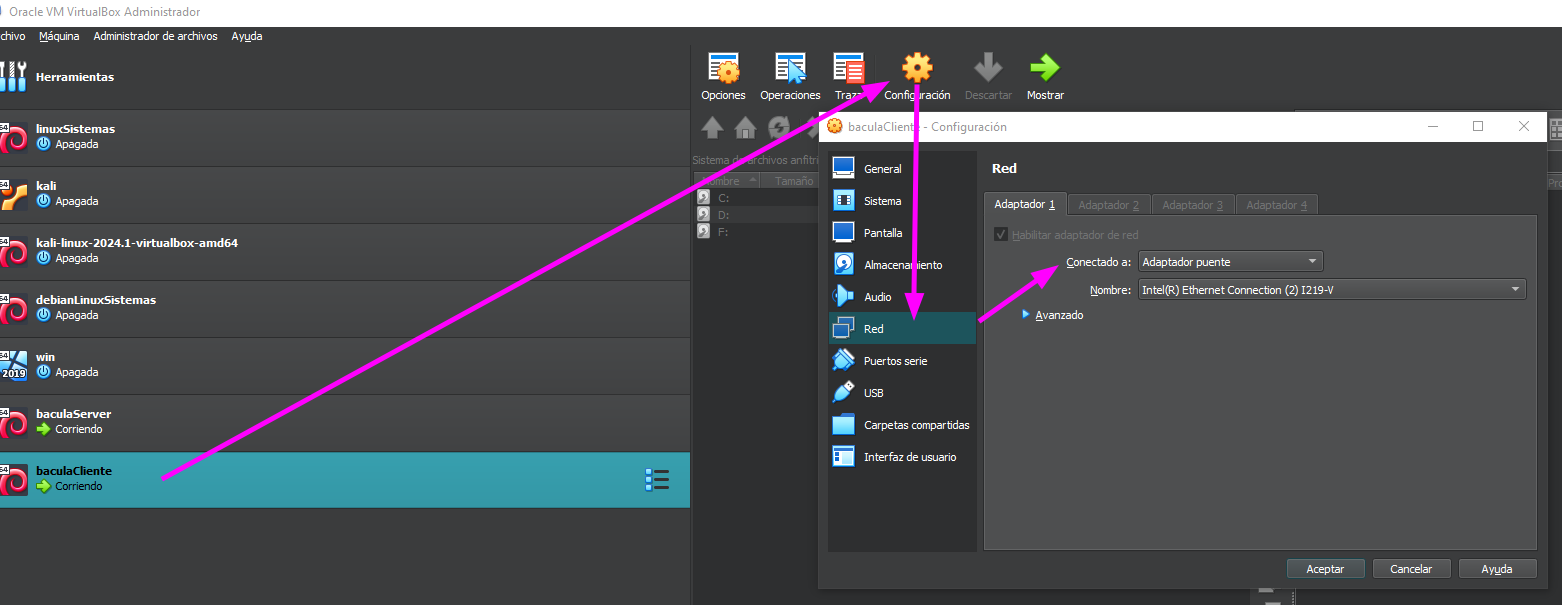
\includegraphics[width=0.5\linewidth]{instalacionBacula/NatAdaptadorPuente.png}
    \caption{Enter Caption}
\end{figure}



%%%%%%%%%%%%%%%%%%%%%%%%%%%%%%%%%%%%%%%%%%%%%%%%
---------------------------------------------
Primero necesitamos añadir los puertos de bacula al firewall
puertos 9101 director 9102 file deamon 9103 storage deamon
para ello usamos los comandos:

sudo ufw allow 9101/tcp
sudo ufw allow 9102/tcp
sudo ufw allow 9103/tcp



\begin{figure}[H]
    \centering
    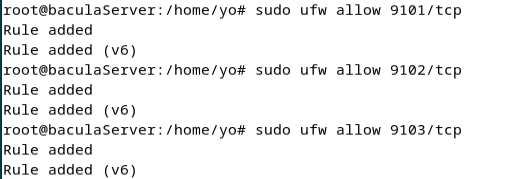
\includegraphics[width=0.5\linewidth]{instalacionBacula/puertosBaCULAufw.png}
    \caption{Enter Caption}
\end{figure}

A continuacion necesitamos tener acceso a los repositorios de bacula, desafortunadamente tienes que estar registrado en su pagina  https://www.bacula.org/ para obtenerlos

\begin{figure}[H]
    \centering
    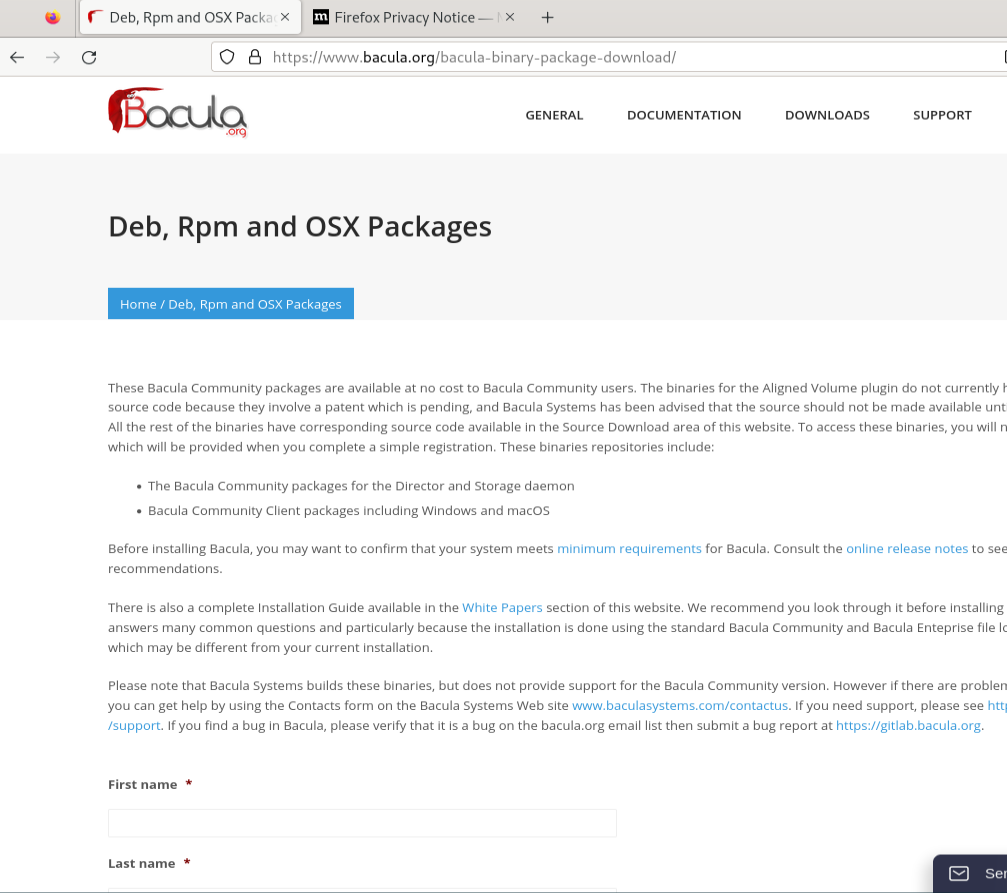
\includegraphics[width=0.5\linewidth]{instalacionBacula/registroBacula.png}
    \caption{Enter Caption}
\end{figure}


Una vez registrados ya podemos acceder a los binarios, para ello vamos a 
debs -> ultima version 15.0.2 -> dist -> bookworm-> main-binary amd -> install


\begin{figure}[H]
    \centering
    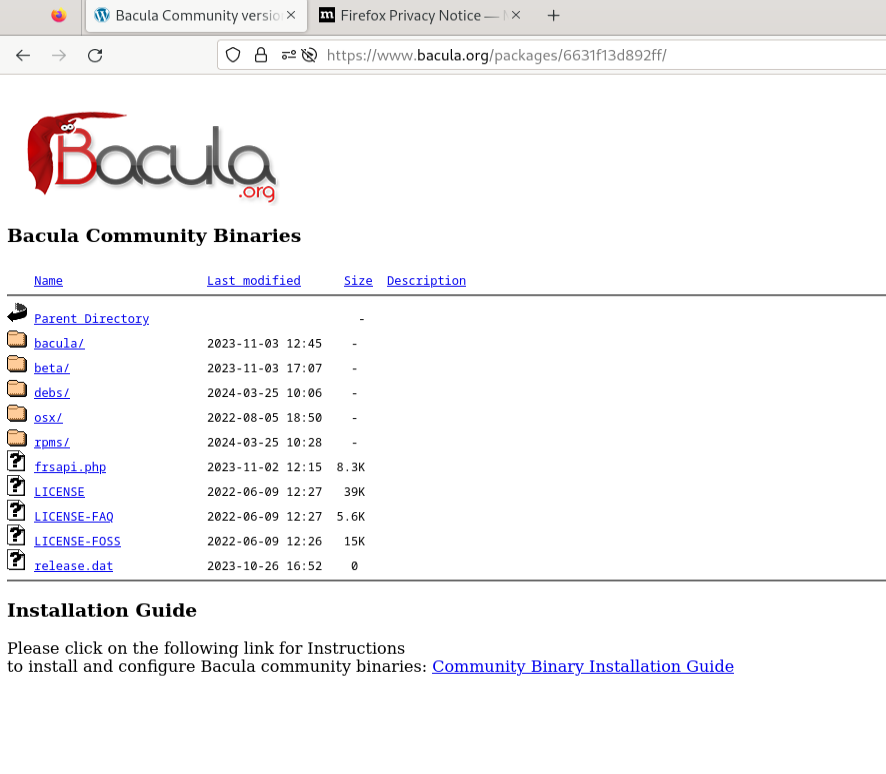
\includegraphics[width=0.5\linewidth]{instalacionBacula/baculapackages.png}
    \caption{Enter Caption}
\end{figure}

Añadimos la clave de verificacion distribucion con los comandos:
  wget https://bacula.org/downloads/Bacula-4096-Distribution-Verification-key.asc
  apt-key add Bacula-4096-Distribution-Verification-key.asc
  

  

\begin{figure}[H]
    \centering
    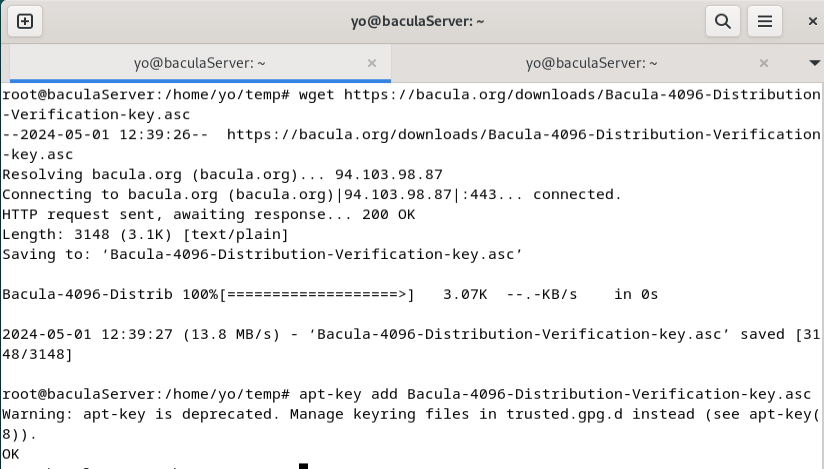
\includegraphics[width=0.5\linewidth]{instalacionBacula/baculaSignature.png}
    \caption{Enter Caption}
\end{figure}

Y los repositorios a sources.list :

\begin{figure}[H]
    \centering
    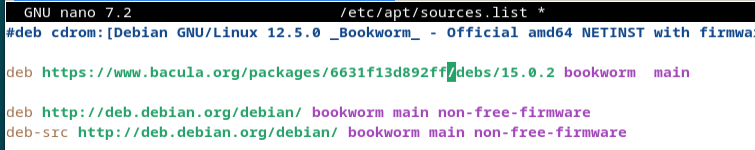
\includegraphics[width=0.5\linewidth]{instalacionBacula/baculaRepositorio.png}
    \caption{Enter Caption}
\end{figure}

Antes de seguir un aspecto importante es que base de datos para el catalogo elegir.
Cuando configuras Bacula para gestionar copias de seguridad, elegir entre MySQL y PostgreSQL para su servicio de catálogo puede depender de varias consideraciones técnicas y de licencia. A continuación, se presenta una comparación detallada:


\begin{table}
    \centering
    \begin{tabular}{ccc}
        Aspecto & MySQL & PostgreSQL\\
        Licencia & GNU GPL, que es más restrictiva en términos de obligaciones de compartir cambios & BSD, más permisiva y flexible para el uso en productos derivados sin compartir el código.\\
        Madurez & Muy maduro y ampliamente adoptado en aplicaciones web y de empresa. & Extremadamente maduro, con un enfoque en características avanzadas y conformidad con SQL.\\
        Desempeño & Generalmente más rápido en operaciones de lectura y carga de trabajo menos complejas. & Excelente en transacciones complejas y operaciones concurrentes de alta integridad.\\
        Características & 	Orientado al rendimiento con características de usabilidad fácil. &Soporta un conjunto más amplio de características SQL, funciones avanzadas y tipos de datos. \\
        Soporte de Datos	& Bueno para manejar grandes volúmenes de datos en sitios menos complejos. & Mejor para manejar complejidades en grandes bases de datos y con requerimientos estrictos. \\
        Seguridad y Confiabilidad & Confiabilidad alta, pero PostgreSQL tiene una reputación superior en robustez y seguridad. & Considerado muy robusto y seguro, con soporte extenso para políticas de seguridad detalladas.\\
        Facilidad de Configuración & Relativamente fácil de configurar y popular en la comunidad con muchos recursos disponibles. & Requiere más configuración inicial pero es altamente personalizable.\\
    \end{tabular}
    \caption{Caption}
\end{table}


Recomendaciones para usar MySQL o PostgreSQL con Bacula:
MySQL: Ideal para entornos donde la velocidad y la simplicidad son prioritarias. Su licencia GPL puede ser adecuada si el proyecto también se distribuirá bajo GPL o cuando la licencia no representa un problema.

PostgreSQL: La mejor opción si se requiere un sistema de gestión de base de datos robusto, con características avanzadas y mejor conformidad con SQL. Su licencia BSD es favorable para incorporar Bacula en productos que no desean estar ligados a las restricciones de GPL.

Yo me decline por postgres por tanto instalamos la base de datos para el catalogo con apt-get install dbconfig-common postgresql y instalmos bacula con postgres mediante apt-get install bacula-postgresql.
\begin{figure}[H]
    \centering
    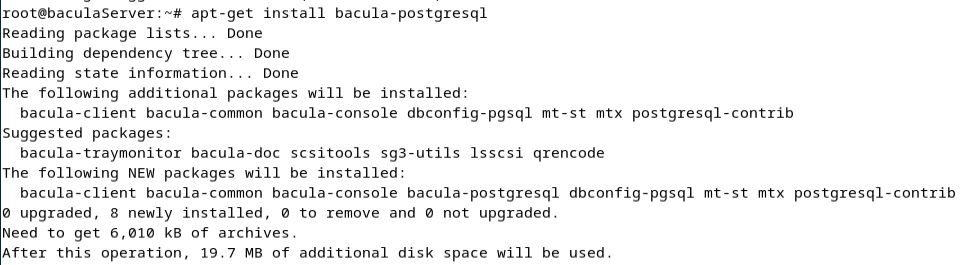
\includegraphics[width=0.5\linewidth]{instalacionBacula/baculapostgesql.png}
    \caption{Enter Caption}
\end{figure}


configuramos baccula con postgresql
\begin{figure}[H]
    \centering
    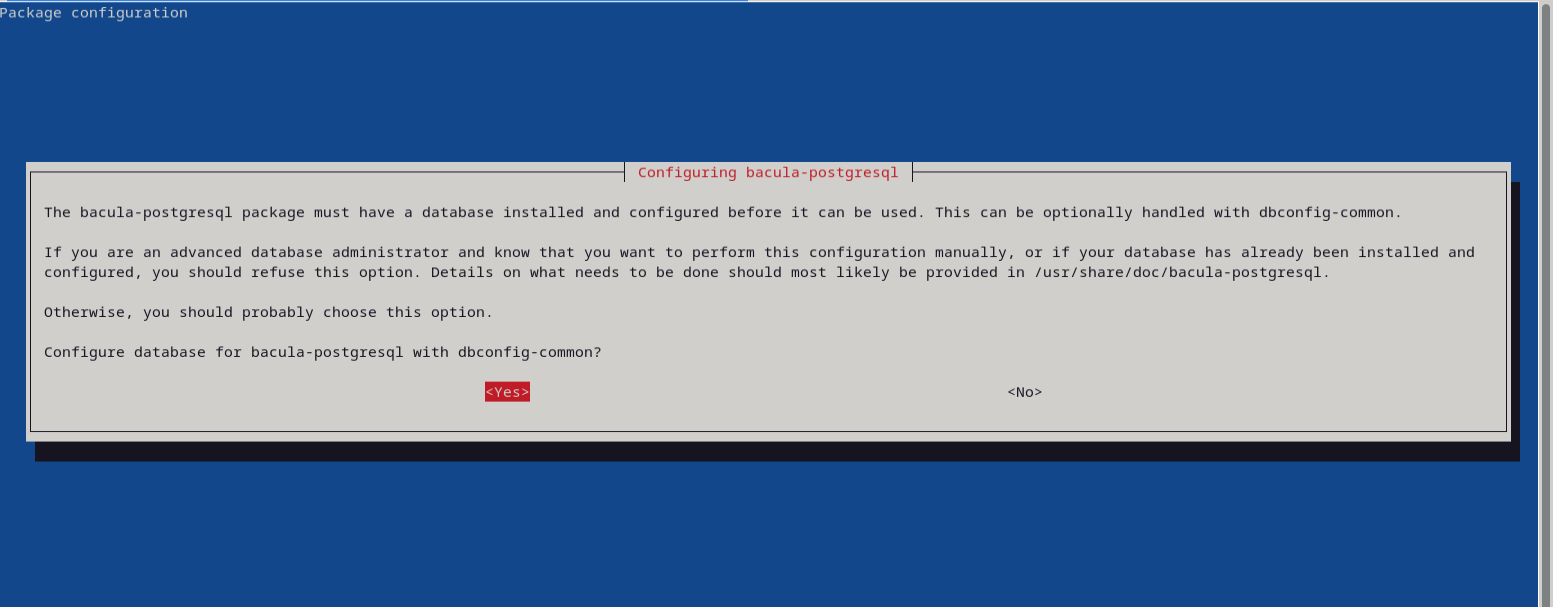
\includegraphics[width=0.5\linewidth]{instalacionBacula/configbaculapostgre.png}
    \caption{Enter Caption}
\end{figure}

Y comprobamos que se instalo correctamente:
\begin{figure}[H]
    \centering
    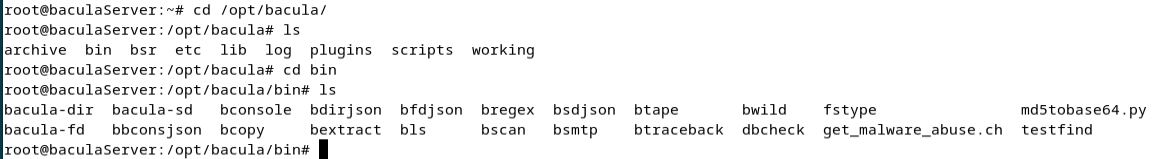
\includegraphics[width=0.5\linewidth]{instalacionBacula/baculadir.png}
    \caption{Enter Caption}
\end{figure}

Y añadimos al path los scripts de bacula con
export PATH=\$PATH:/opt/bacula/bin


\newpage
%%%%%%%%%%%%%%%%%%%%%%%%%%%%%%%%%%%%%%%%%%%%%%%%%%%
----------------------------------

instalar webmin


primero instalamos apache:

\begin{figure}[H]
    \centering
    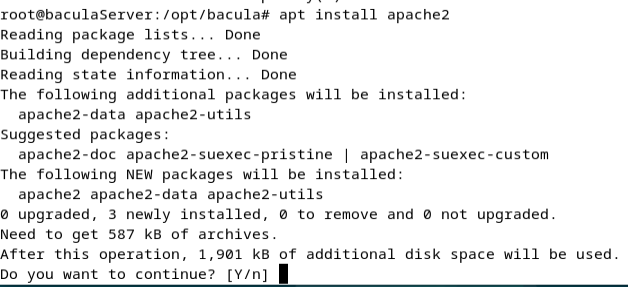
\includegraphics[width=0.5\linewidth]{instalacionBacula/apache2.png}
    \caption{Enter Caption}
\end{figure}


añadimos http y https al firewall

sudo ufw allow 80/tcp
sudo ufw allow 443/tcp


\begin{figure}[H]
    \centering
    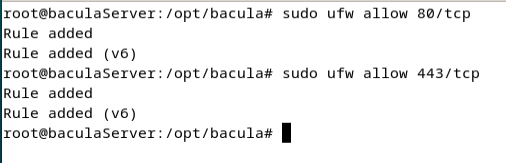
\includegraphics[width=0.5\linewidth]{instalacionBacula/htpsFirewall.png}
    \caption{Enter Caption}
\end{figure}



PARA INSTALAR  webmin 
curl -o setup-repos.sh https://raw.githubusercontent.com/webmin/webmin/master/setup-repos.sh
sh setup-repos.sh

\begin{figure}[H]
    \centering
    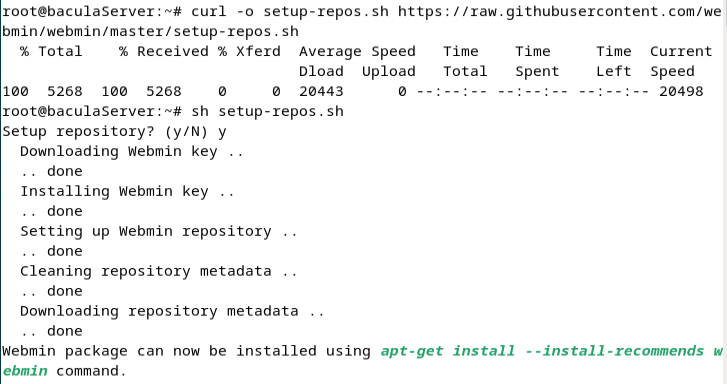
\includegraphics[width=0.5\linewidth]{instalacionBacula/CURLwebmin.png}
    \caption{Enter Caption}
\end{figure}


apt-get install webmin --install-recommends


\begin{figure}[H]
    \centering
    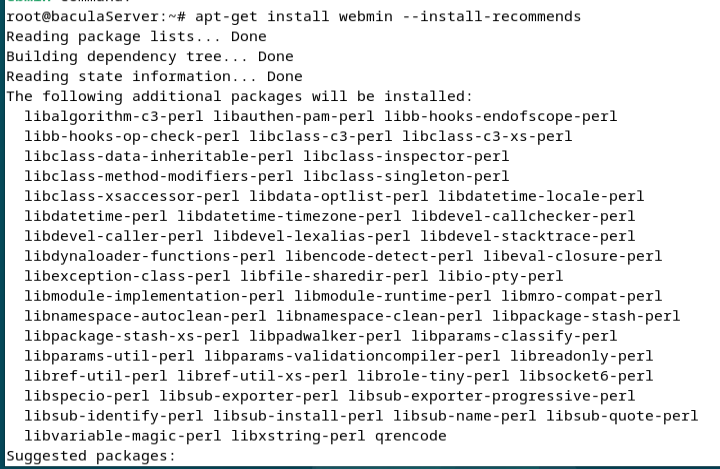
\includegraphics[width=0.5\linewidth]{instalacionBacula/instalWebminn.png}
    \caption{Enter Caption}
\end{figure}


y añadimos el puerto 10000 al firewal
\begin{figure}[H]
    \centering
    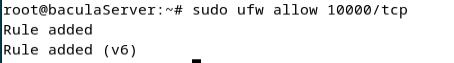
\includegraphics[width=0.5\linewidth]{instalacionBacula/puerto10000.png}
    \caption{Enter Caption}
\end{figure}


Y ahora ya podemos acceder la consola de webmin en el navegador:

\begin{figure}[H]
    \centering
    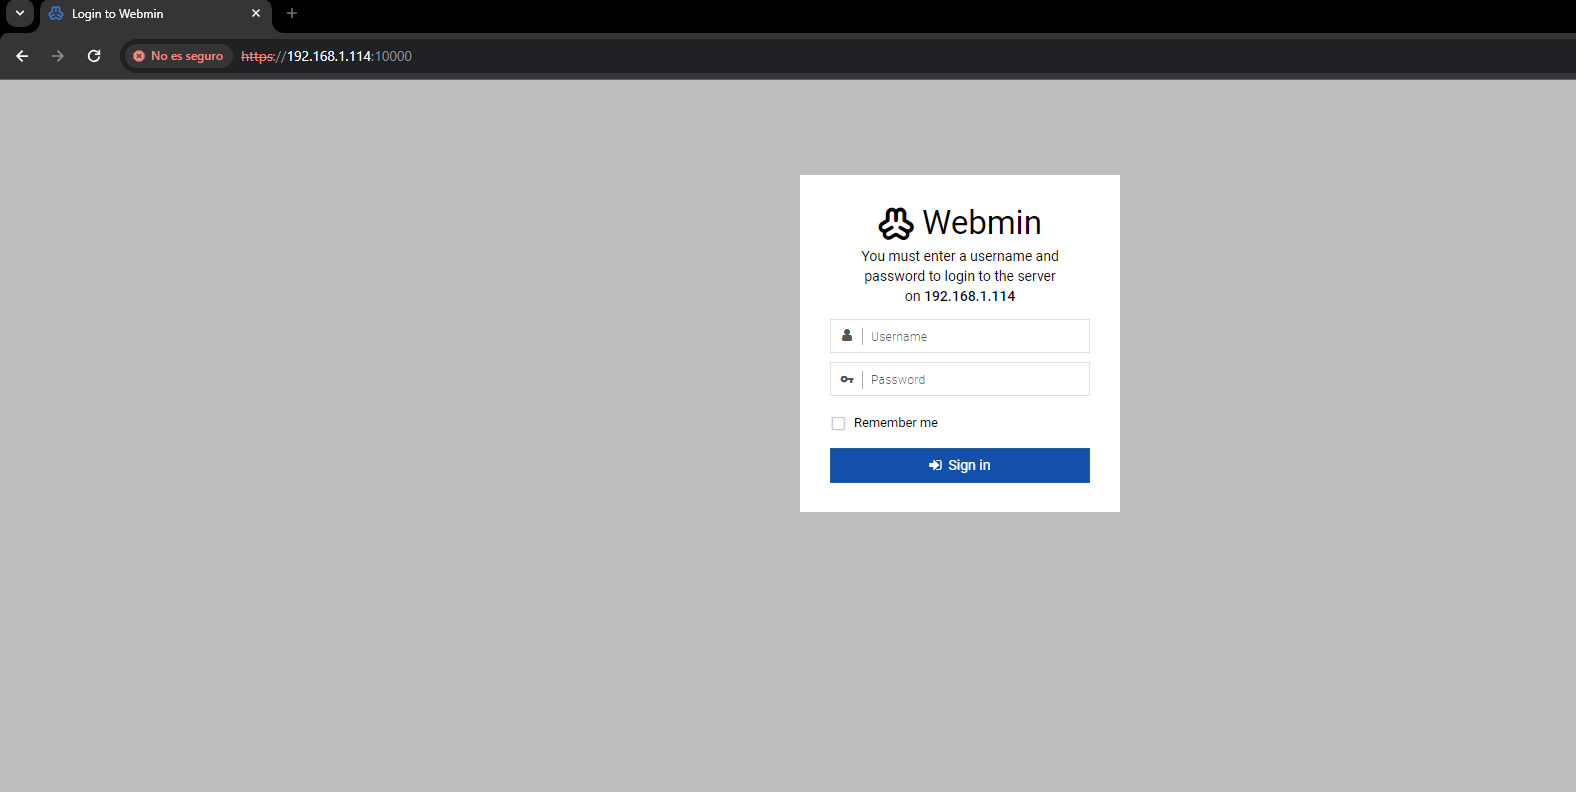
\includegraphics[width=0.5\linewidth]{instalacionBacula/webmin.png}
    \caption{Enter Caption}
\end{figure}


ahora podemos configurar el modulo de bacula en webmin 
añadimos los directorios de bacula a webmin

Bacula configuration directory
/opt/bacula/etc
Full path to bextract command
/opt/bacula/bin/bextract
Full path to bls command
/opt/bacula/bin/bls
Full path to btape command
/opt/bacula/bin/btape

\begin{figure}[H]
    \centering
    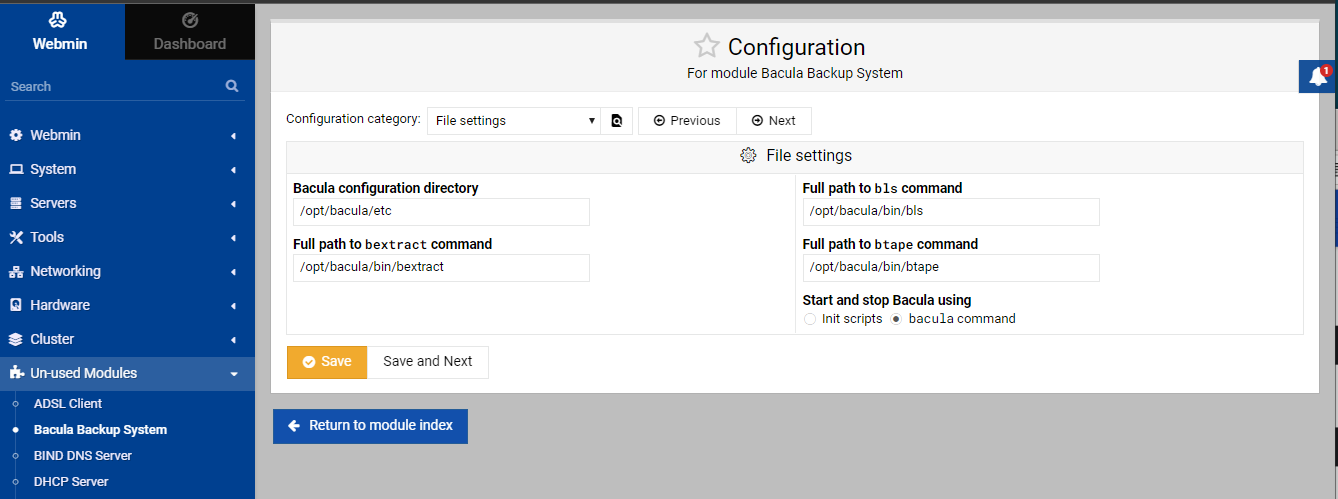
\includegraphics[width=0.5\linewidth]{instalacionBacula/pathwebmin.png}
    \caption{Enter Caption}
\end{figure}


si diese error habria que en el archivo de configuracion pg\_hba.conf de postgesql/15/main y darle/cambiarle permisos de autentificacion a nuestro usuario de bacula para ello

\# TYPE  DATABASE        USER            ADDRESS                 METHOD
local   all             all                                     md5

\begin{figure}[H]
    \centering
    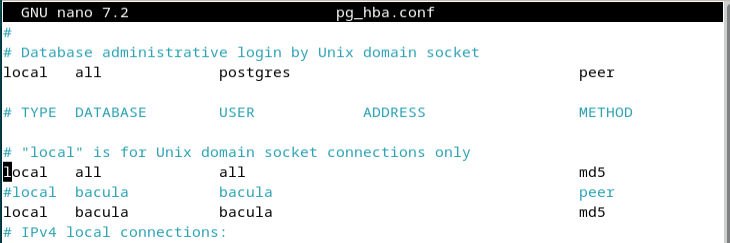
\includegraphics[width=0.5\linewidth]{instalacionBacula/md5postgesql.png}
    \caption{Enter Caption}
\end{figure}

guardamos y reiniciamos el servicio de postgresql
systemctl restart postgresql

%%%%%%%%%%%%%%%%%%%%%%%%%%%%%%%%
-------------------------

configuracion del almacenamiento local

creamos un directorio para almacenamiento 
con mkdir backups

y le damos propiedad a bacula sobre esa direccion con 

\begin{figure}[H]
    \centering
    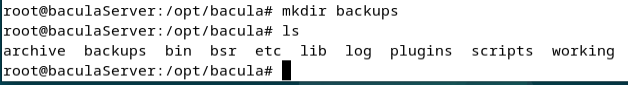
\includegraphics[width=0.5\linewidth]{instalacionBacula/mkdirbackups.png}
    \caption{Enter Caption}
\end{figure}



\begin{figure}[H]
    \centering
    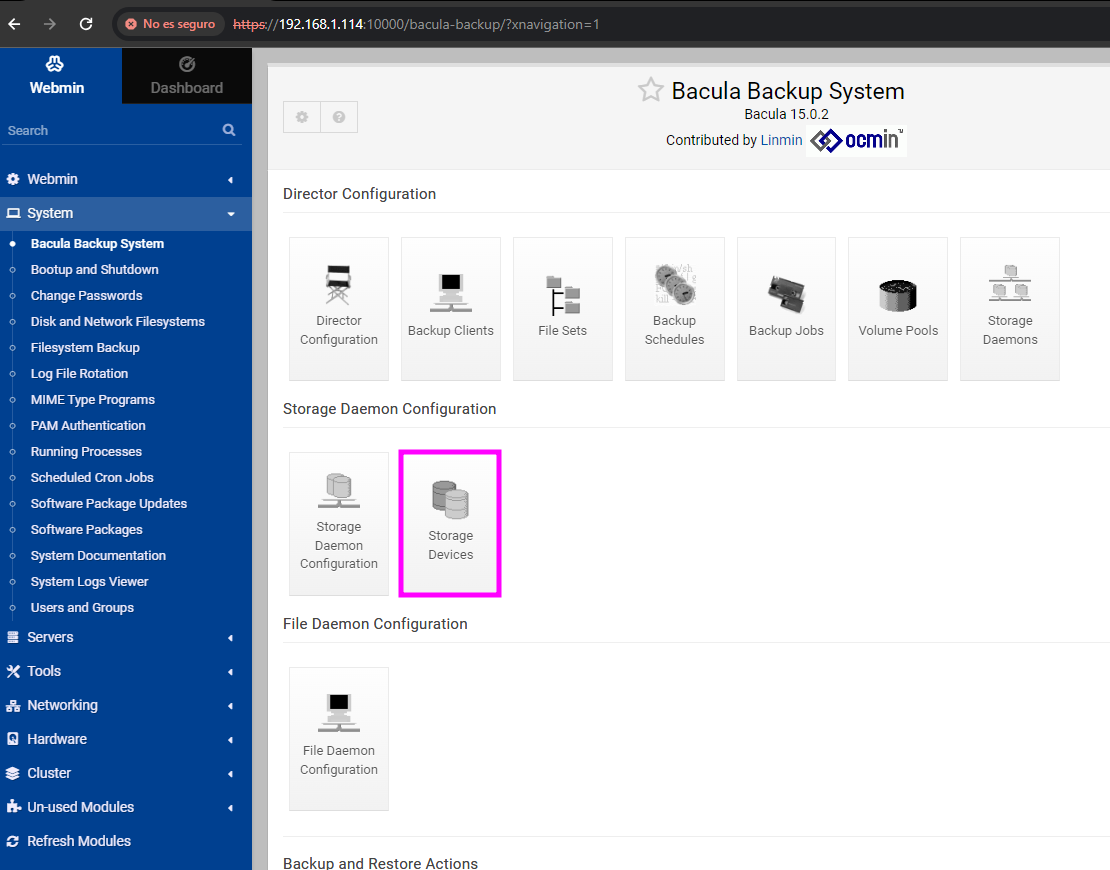
\includegraphics[width=0.5\linewidth]{instalacionBacula/STO.png}
    \caption{Enter Caption}
\end{figure}


NOS ENCONTRAMOS UNOS STORAGES DEVICES QUE VIENEN DEFAULT
PERO CREAMOS UNO NUEVO
\begin{figure}[H]
    \centering
    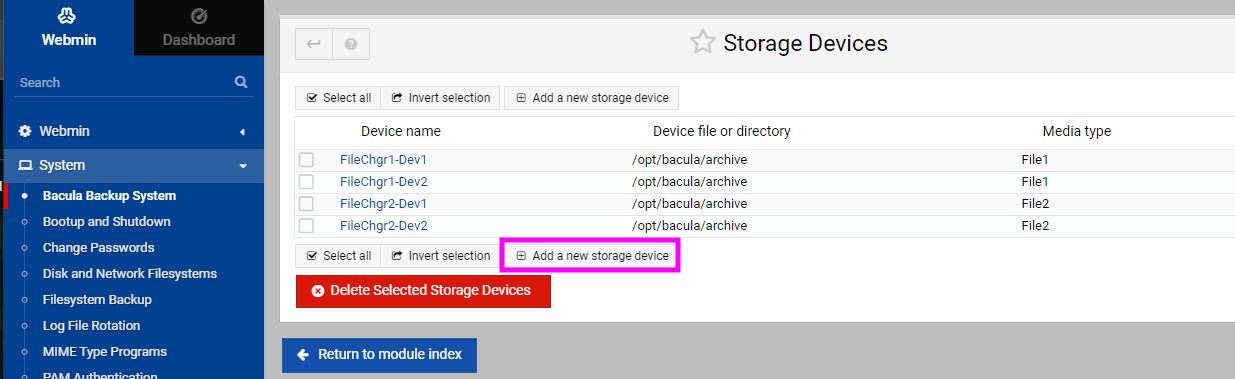
\includegraphics[width=0.5\linewidth]{instalacionBacula/NSD.png}
    \caption{Enter Caption}
\end{figure}

(explcar estos:)
Storage device name
    localBackups
Archive device or directory
    /otp/bacula/backups
Media type name
    localBackups

\begin{figure}[H]
    \centering
    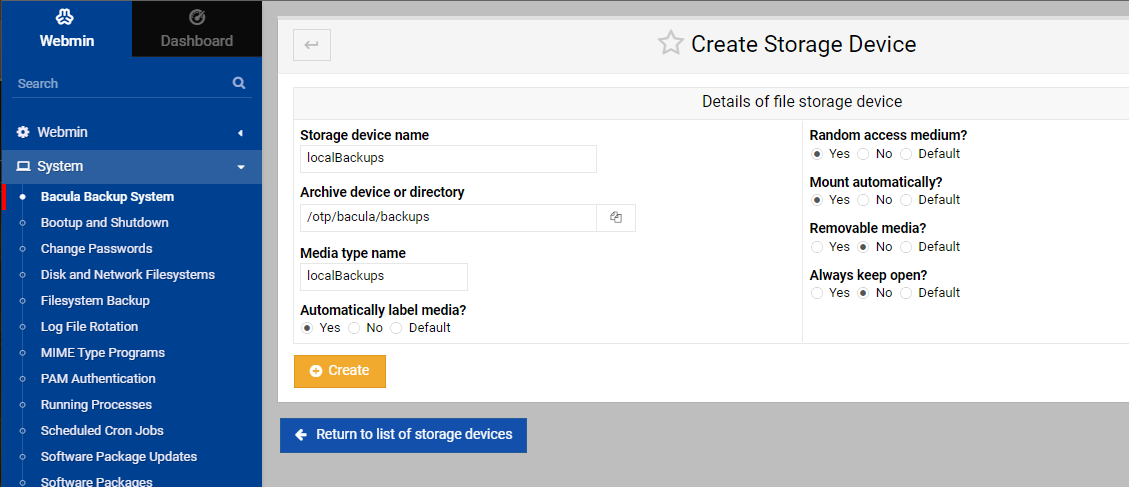
\includegraphics[width=0.5\linewidth]{instalacionBacula/localbac.png}
    \caption{Enter Caption}
\end{figure}


en este directorio nos van a ver los archivos sueltos de los backups que van a ir tomando.

Van a ver un archivo donde en él va a estar de manera cifrada toda la información que ustedes vayan

respaldando con lo cual si alguien les ganar acceso al servidor local simplemente verían una cosa así.

Eso sería todo lo que vería en un archivo solo y nada de información.
configuramos en bacula el uso de almacenamiento local


ahora creamos un storage deamon
\begin{figure}[H]
    \centering
    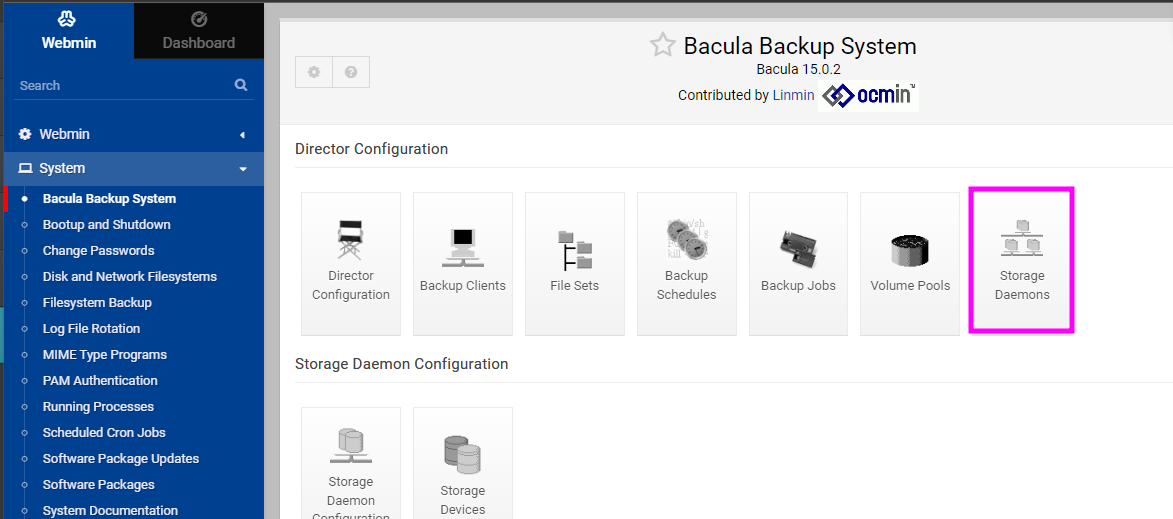
\includegraphics[width=0.5\linewidth]{instalacionBacula/stdeamon.png}
    \caption{Enter Caption}
\end{figure}


añadimo un nuevo storage deamon
\begin{figure}[H]
    \centering
    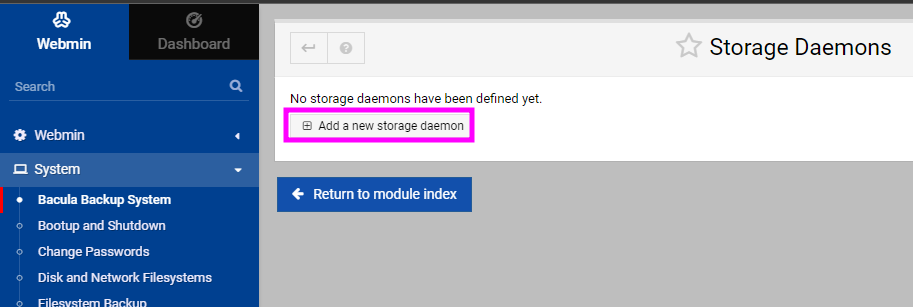
\includegraphics[width=0.5\linewidth]{instalacionBacula/newsd.png}
    \caption{Enter Caption}
\end{figure}

si ponemos el nombre del servidor tenemos que enseñarle a todos los clientes que vamos a realizarles copias de seguridad que puedan resolver el servidor por nombre en nuestro caso como no tenemos un servidor de DNS vamos a poner acá la dirección IP del servidor de backup para ahorrarnos el trabajo de los clientes tener que andar editando el archivo hoost entonces vamos a poner directamente la IP del servidor 

Details of remote storage daemon
(habria que explicar estas opciones)
-Storage daemon name
StorageDeamon
-Bacula SD password
1234
-Hostname or IP address
192.168.1.114
-Bacula SD port
9103
-Storage device name

localBackups
 

-Media type name
localBackups
-Maximum concurrent jobs
20


\begin{figure}[H]
    \centering
    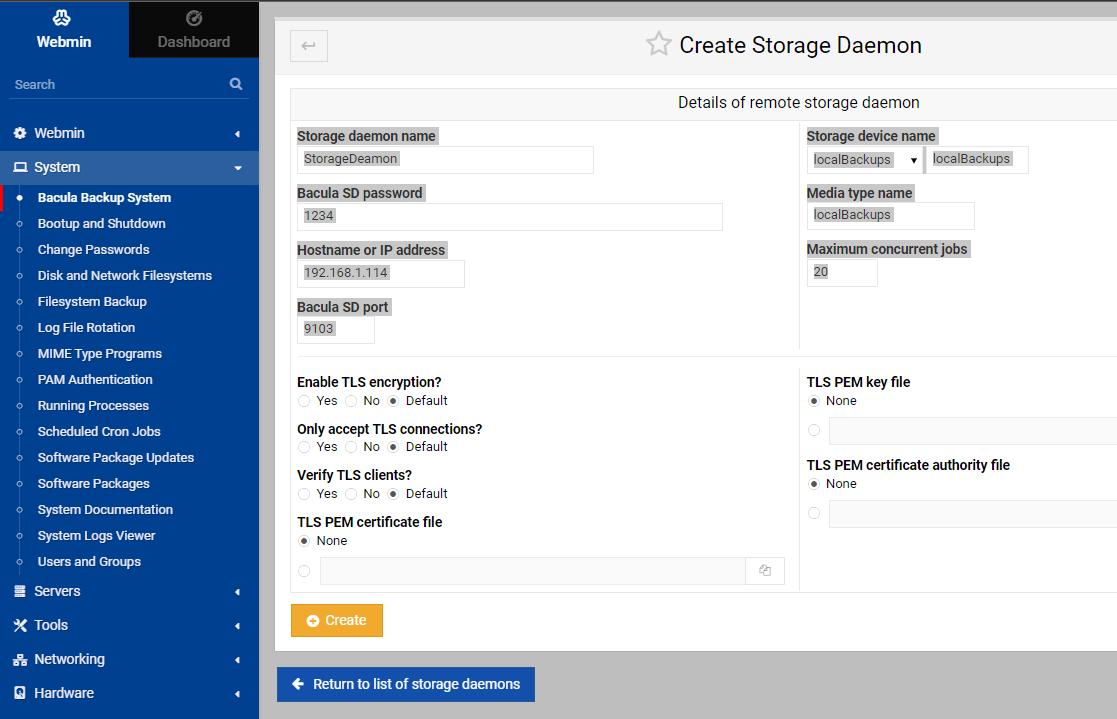
\includegraphics[width=0.5\linewidth]{instalacionBacula/storagedeamonWebmin.png}
    \caption{Enter Caption}
\end{figure}
para mejorar la seguridad de las copias de seguridad agregando certificados y habilitando las comunicaciones TLS.

Y ya tendriamos el storage deamon:
\begin{figure}[H]
    \centering
    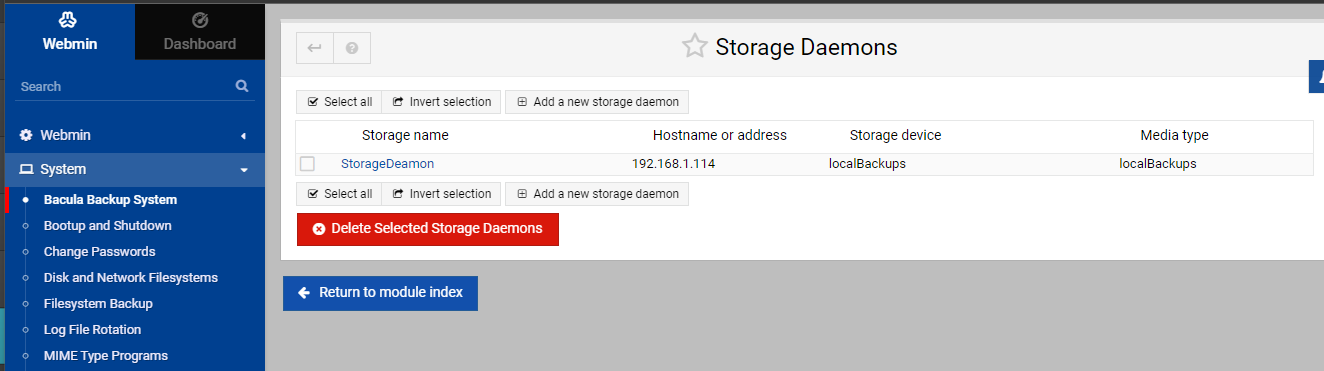
\includegraphics[width=0.5\linewidth]{instalacionBacula/sdwebminaa.png}
    \caption{Enter Caption}
\end{figure}





por ultimo cremos nuestro propio pool de volumenes:

\begin{figure}[H]
    \centering
    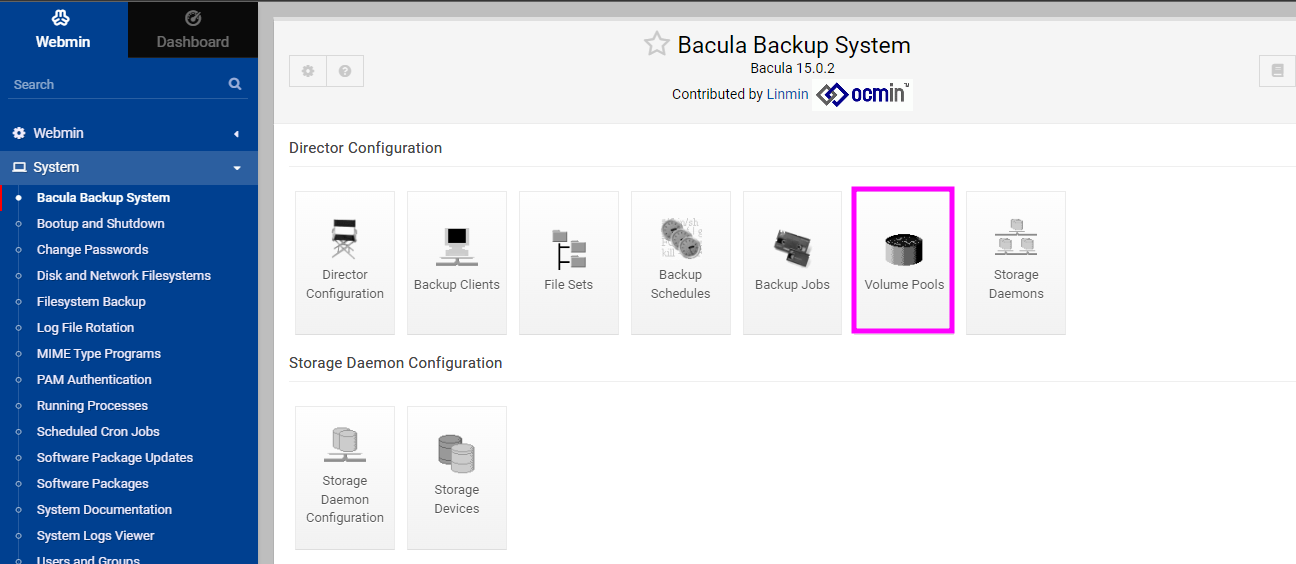
\includegraphics[width=0.5\linewidth]{instalacionBacula/pollv.png}
    \caption{Enter Caption}
\end{figure}



\begin{figure}[H]
    \centering
    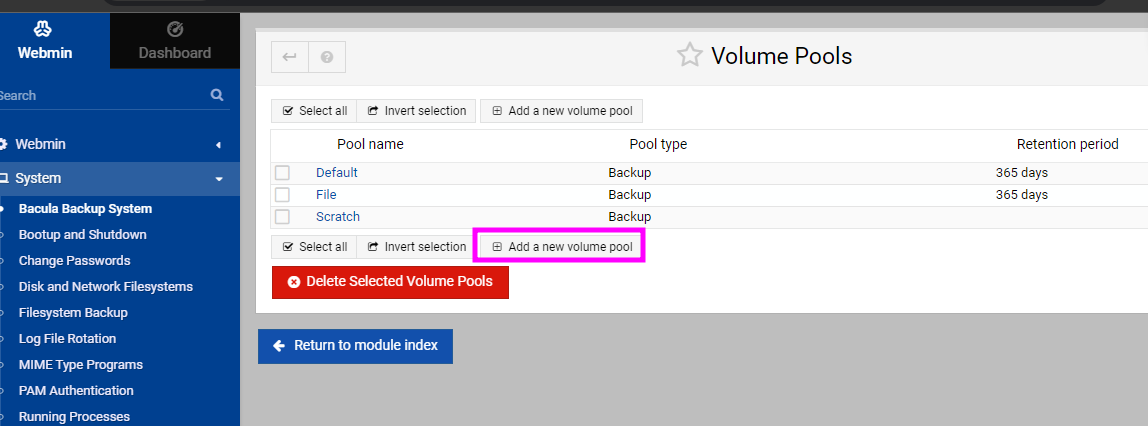
\includegraphics[width=0.5\linewidth]{instalacionBacula/pool22.png}
    \caption{Enter Caption}
\end{figure}

ahora para  configurar el volumen:
Details of backup volume pool

(abria que explcar estas opciones)
-Volume pool name
Pool1
-Volume pool type

Backup
-Maximum jobs per volume

  Unlimited 
 
  
-Volume retention period
    365 days
    
-Automatically recycle volumes?

  Yes 
 
  Default 
-Prune expired volumes?

  Yes 
 
 
  Default 
-Automatically label volumes prefix
Backup
-Maximum volume size 
3G

\begin{figure}
    \centering
    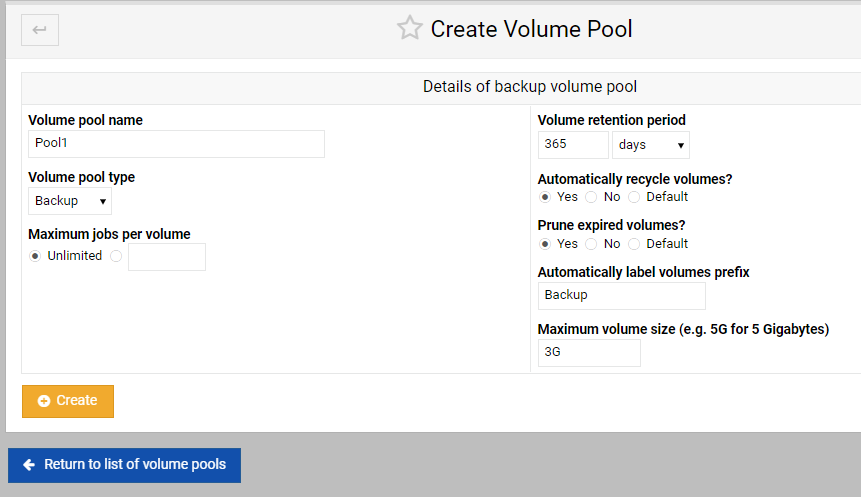
\includegraphics[width=0.5\linewidth]{instalacionBacula/createVolumePool.png}
    \caption{Enter Caption}
\end{figure}


Pueden ponerlo de 15 días de tres meses de un año.

Esto lo vamos a ir viendo más en detalle adelante cuando hablemos de estrategias de backup.

Y por último podemos ponerle un límite al tamaño que cada uno de esos archivos puede tener.

Vamos a ponerle 10 siglas cada uno de estos archivos donde vaya guardando los backups no puede exceder los 3 gigas.

Esto también es parte de una estrategia de backup.

Por el momento vamos a dejarlo así para que podamos hacer una práctica simple de backup y después lo

abordaremos cuando vemos estrategias.

%%%%%%%%%
------------------------------------- 
Instalar bacula client en Linux

añadimos el file demon baculhel puerto 9102 al firewall 
\begin{figure} [H]
    \centering
    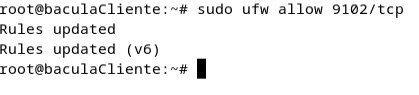
\includegraphics[width=0.5\linewidth]{instalacionBacula/9102alfirewall.png}
    \caption{Enter Caption}
\end{figure}


al igual que antes añadimos los repositorios de bacula


ahora instalamos el cliente de bacula:
apt install bacula-client

y como vemos se instalo correctamente:

\begin{figure}[H]
    \centering
    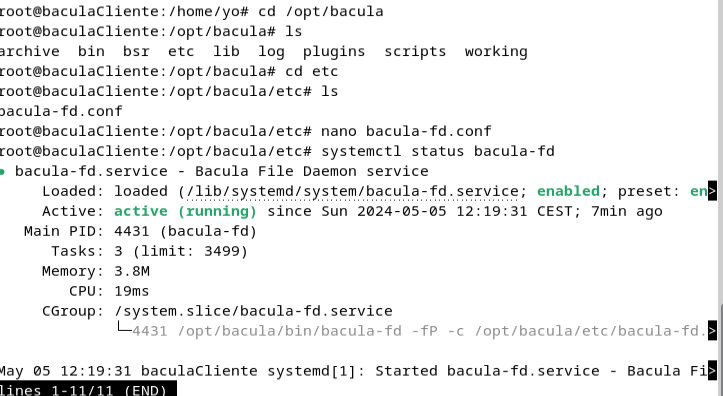
\includegraphics[width=0.5\linewidth]{instalacionBacula/baculaClienteinstalacion2.png}
    \caption{Enter Caption}
\end{figure}

y editamos el archivo /opt/bacula/etc/bacula-fd.conf

\begin{figure}[H]
    \centering
    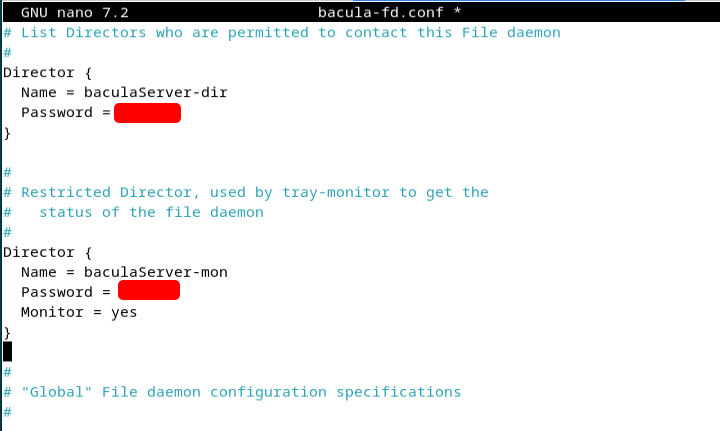
\includegraphics[width=0.5\linewidth]{instalacionBacula/baculaFDcongf.png}
    \caption{Enter Caption}
\end{figure}

%%%%%%%%%%%%%%
--------------------
realizar backup

necesitamos definir lo siguiente:

definir que es lo que vamos a respaldar
definir cuando lo vamos a respaldar
agregar a quien  vamos a respaldar
crear el  job 
y ejecutar el job




creamos un fileset en webmin

\begin{figure}[H]
    \centering
    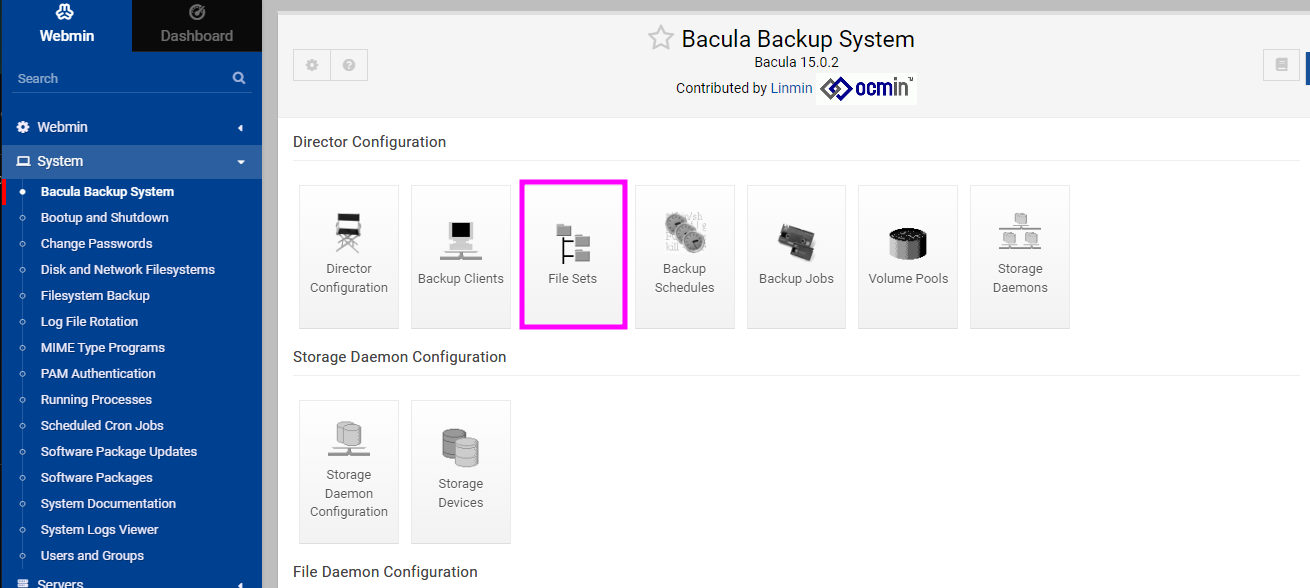
\includegraphics[width=0.5\linewidth]{instalacionBacula/filesetwebmin.png}
    \caption{Enter Caption}
\end{figure}

hay dos fileset creados durante la instalacion

\begin{figure}[H]
    \centering
    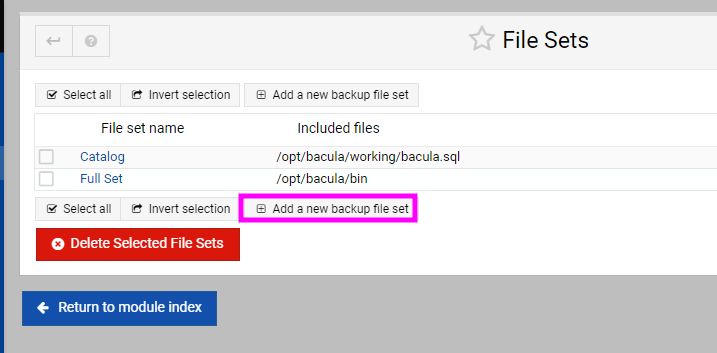
\includegraphics[width=0.5\linewidth]{instalacionBacula/cpropiofileset.png}
    \caption{Enter Caption}
\end{figure}


 reutilizar el Falset en sus diferentes definiciones de Jobs o pueden crear un Falset por cada cliente.

Esto es decisión y gusto de cada uno.

Vamos a poner md5 de para que de esta manera se asegure de que lo que está copiando es una copia fiel

va a comparar las hash MD5 


File set name
ClienteDebian1Archivos
Files and directories to backup
/etc
/root
/home
File signature type
MD5

Files and directories to skip


Compression type

<Default compression level>
Limit backup to one filesystem?

  Yes 
 
  No 
 
  Default 


  \begin{figure}[H]
      \centering
      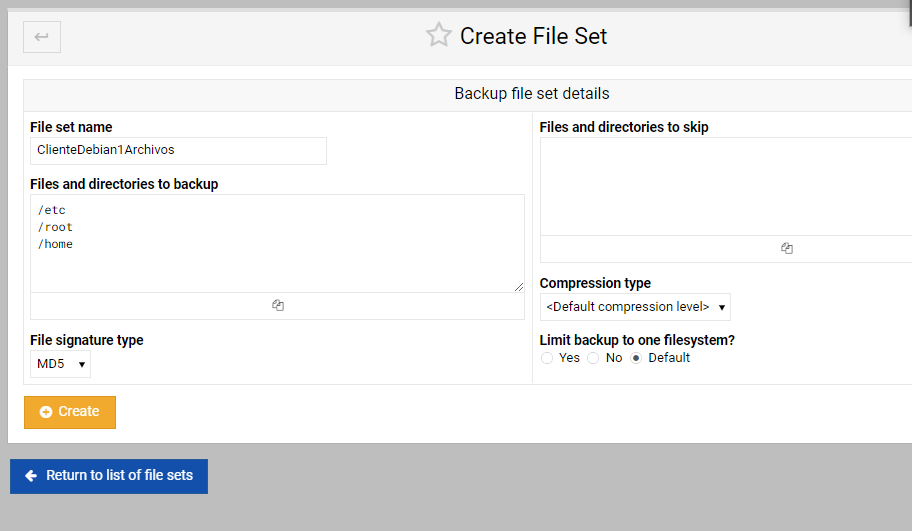
\includegraphics[width=0.5\linewidth]{instalacionBacula/createrfilesett.png}
      \caption{Enter Caption}
  \end{figure}


ahora creamos un schedule:
\begin{figure}[H]
    \centering
    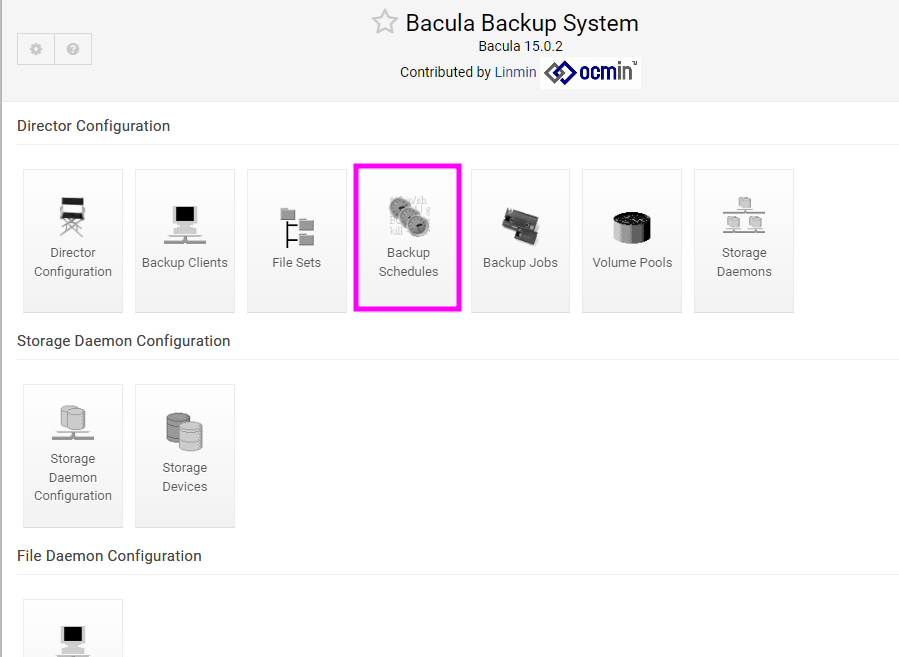
\includegraphics[width=0.5\linewidth]{instalacionBacula/schedule.png}
    \caption{Enter Caption}
\end{figure}

hay ya 2 que vienen con el sistema:

Schedule name	Run levels and times
WeeklyCycle	Full 1st sun at 23:05 , Differential 2nd-5th sun at 23:05 , ...
WeeklyCycleAfterBackup	Full sun-sat at 23:10

pero vamos a crear uno nuevo

\begin{figure}[H]
    \centering
    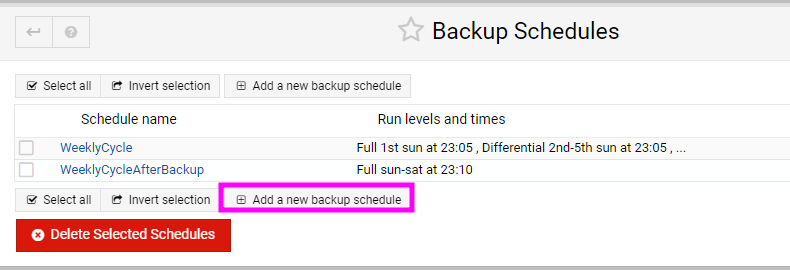
\includegraphics[width=0.5\linewidth]{instalacionBacula/newBackupSchedules.png}
    \caption{Enter Caption}
\end{figure}

aqui nos da las tres opciones de backup, full, partial o diferencial, sobre que volumen hacerlo, y cada cuanto hacerlo:

\begin{figure}[H]
    \centering
    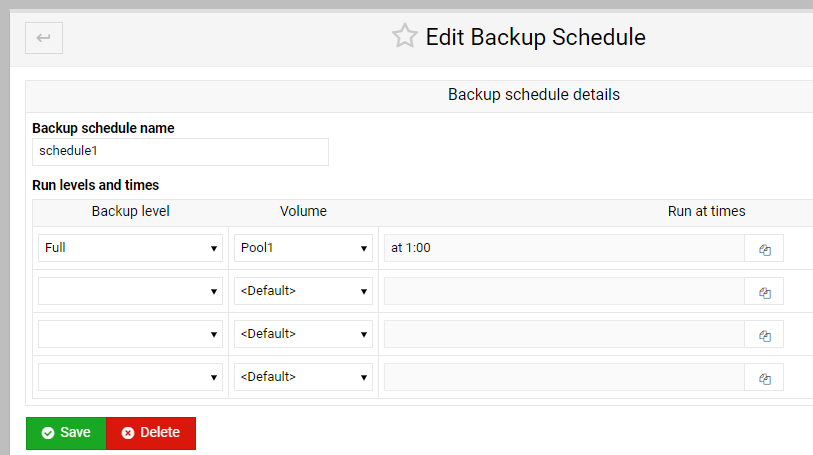
\includegraphics[width=0.5\linewidth]{instalacionBacula/editbuckupschedule.png}
    \caption{Enter Caption}
\end{figure}






ahora necesitamos selecionar a quien vamos a backupear
\begin{figure}[H]
    \centering
    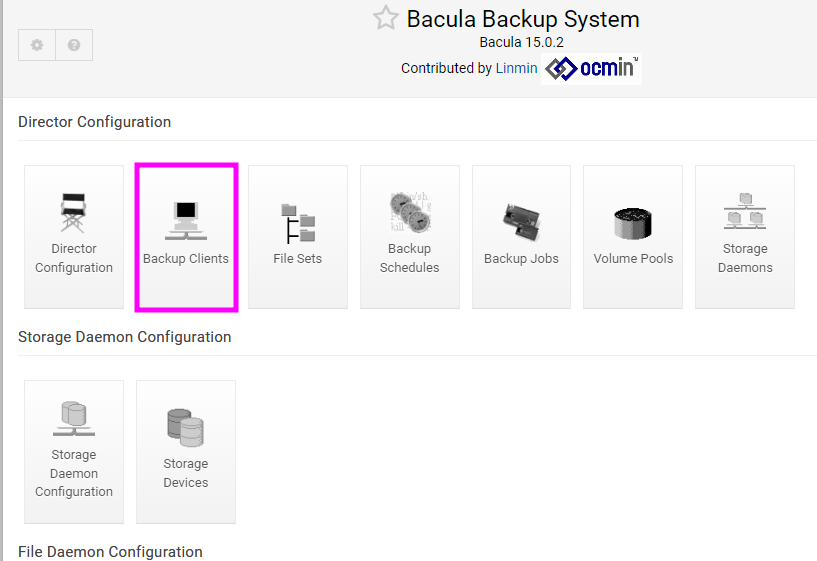
\includegraphics[width=0.5\linewidth]{instalacionBacula/asdasdas.png}
    \caption{Enter Caption}
\end{figure}

de momento solo esta el propio server bacula que se autoagrega en la instalacion, añadimos un nuevo cliente:

\begin{figure}[H]
    \centering
    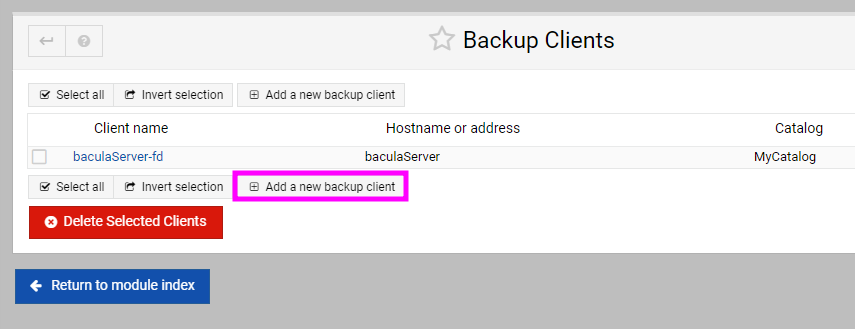
\includegraphics[width=0.5\linewidth]{instalacionBacula/addnewbuckupclient.png}
    \caption{Enter Caption}
\end{figure}


ahora necesitamos definir los Details of client to be backed up
estas opciones son:
-Client FD name
baculaCliente-fd
-Bacula FD password

-Hostname or IP address
192.168.1.116
-Bacula FD port
9102
-Catalog to use

MyCatalog
-Prune expired jobs and files?

  Yes 
 
  No 
 
  Default 
-Keep backup files for
1 months
-Keep backup jobs for
1 months


\begin{figure}[H]
    \centering
    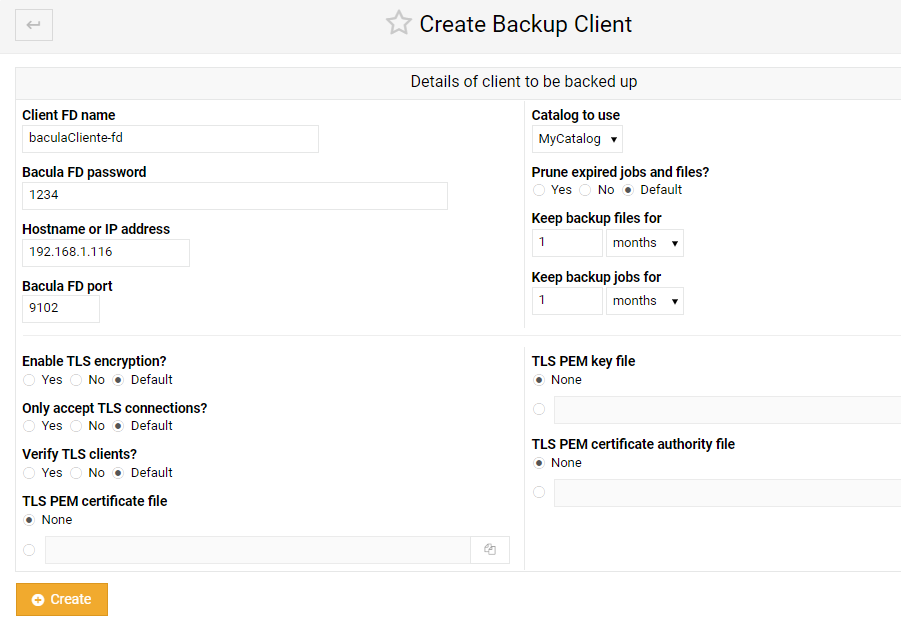
\includegraphics[width=0.5\linewidth]{instalacionBacula/detalesclienteparabuckup.png}
    \caption{Enter Caption}
\end{figure}

ademas podemos añadir encriptacion tls


Ahora podemos crear y ejecutar un job:

\begin{figure}[H]
    \centering
    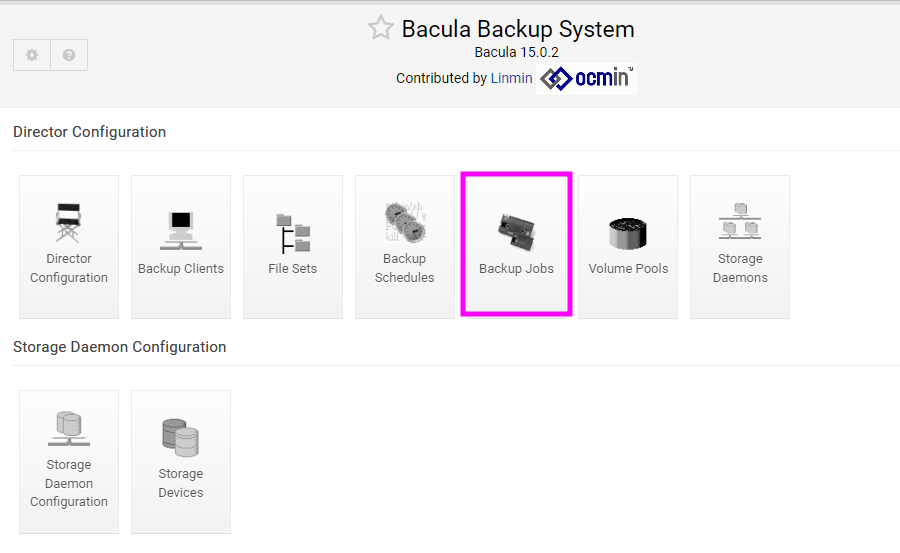
\includegraphics[width=0.5\linewidth]{instalacionBacula/createJOB.png}
    \caption{Enter Caption}
\end{figure}

aqui hay una serie de jobs que vienen por default:

Job name	Defaults?	Job type	Client to backup	File set to backup	Backup schedule
BackupCatalog	No	Default	Default	Catalog	WeeklyCycleAfterBackup
BackupClient1	No	Default	Default	Default	Default
DefaultJob	Yes	Backup	baculaServer-fd	Full Set	WeeklyCycle
RestoreFiles	No	Restore	baculaServer-fd	Full Set	Default

creamos uno nuevo

\begin{figure}[H]
    \centering
    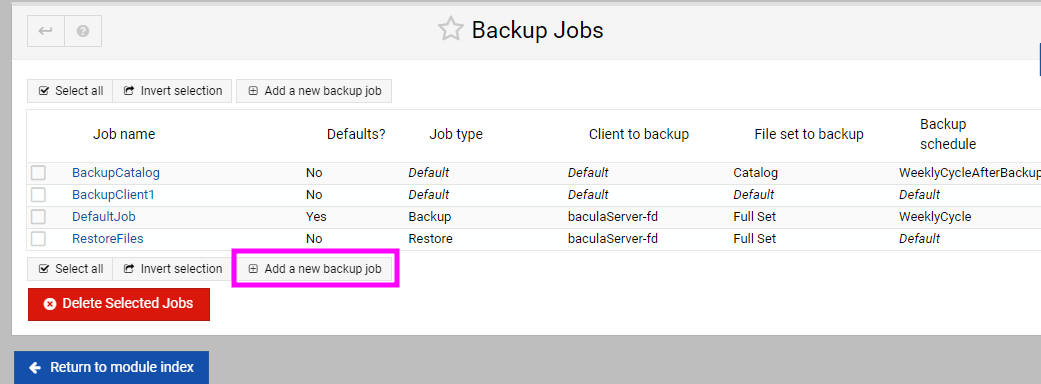
\includegraphics[width=0.5\linewidth]{instalacionBacula/createnewjob.png}
    \caption{Enter Caption}
\end{figure}

y definimos los detalles del job:
\begin{figure}[H]
    \centering
    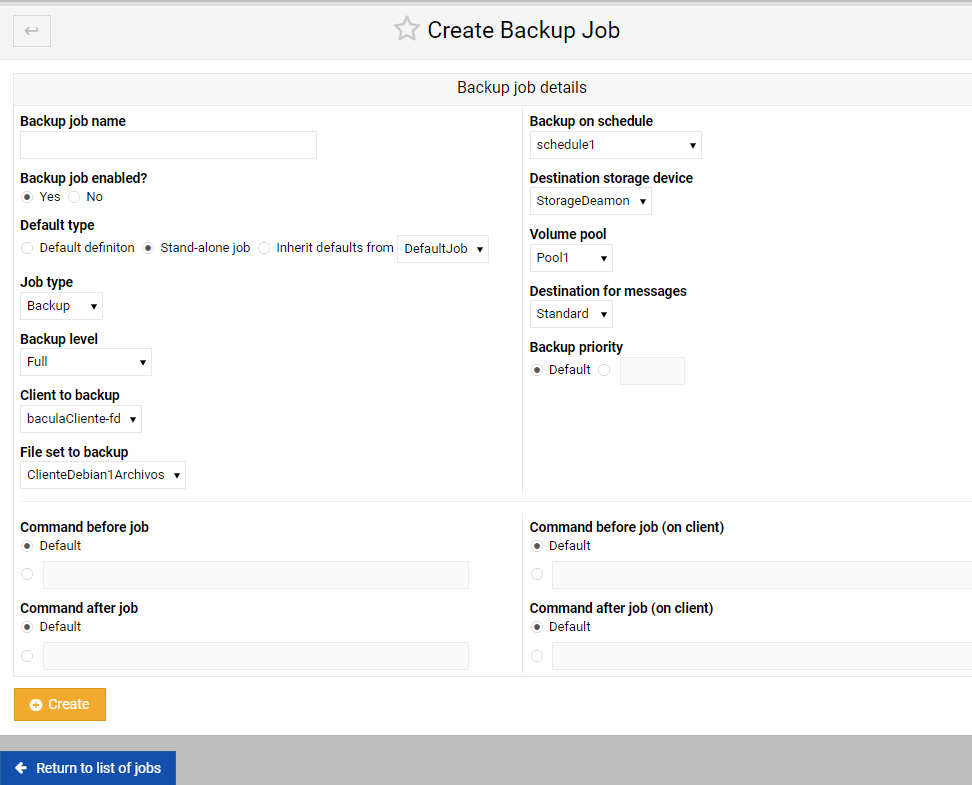
\includegraphics[width=0.5\linewidth]{instalacionBacula/Backupjobdetails.png}
    \caption{Enter Caption}
\end{figure}
estas opciones son:
-Backup job enabled?

  Yes 
 
  No 
-Default type

  Default definiton 
 
  Stand-alone job 
 
  Inherit defaults from 

  DefaultJob
-Job type

Backup
Backup level

Full

-Client to backup

baculaCliente-fd
-File set to backup

ClienteDebian1Archivos
-Backup on schedule

schedule1
-Destination storage device

StorageDeamon
-Volume pool

Pool1
-Destination for messages

Standard
-Backup priority

  Default 
 
  
tambien se pueden ejecutar comandos antes o despues del job en el cliente o el servidor



para ejecutar un job (de forma manual)

\begin{figure}[H]
    \centering
    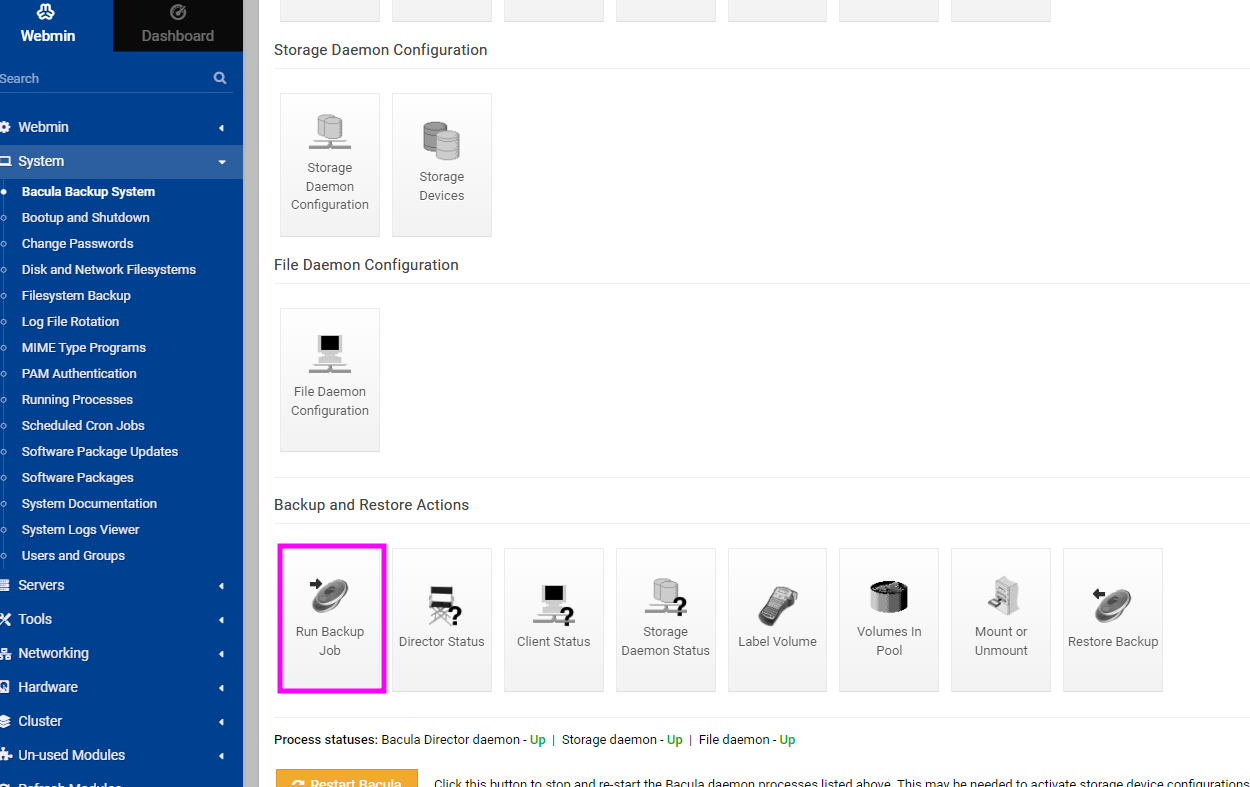
\includegraphics[width=0.5\linewidth]{instalacionBacula/runbackupjonbb.png}
    \caption{Enter Caption}
\end{figure}

elegimos el job que queremos ejecutar y hacemos backup now
\begin{figure}[H]
    \centering
    \includegraphics[width=0.5\linewidth]{instalacionBacula/backupnoww.png}
    \caption{Enter Caption}
\end{figure}

y nos devuelve una salida como la siguiente:
\begin{figure}[H]
    \centering
    \includegraphics[width=0.5\linewidth]{instalacionBacula/salidajob1.png}
    \caption{Enter Caption}
\end{figure}

%%%%%%%%%%%%%%%%%%%%%%
---------------------------
Restore en linux cliente

para ello he creado 5 archivos txt y he obtenido el md5 sum de 2 y 3 que los voy a borrar:

\begin{figure}[H]
    \centering
    \includegraphics[width=0.5\linewidth]{instalacionBacula/5ARCHIVOS.png}
    \caption{Enter Caption}
\end{figure}

Primero hago el backup en bacula:
\begin{figure}[H]
    \centering
    \includegraphics[width=0.5\linewidth]{instalacionBacula/backup0002.png}
    \caption{Enter Caption}
\end{figure}

eliminamos los archivos 2 y 3:

\begin{figure}[H]
    \centering
    \includegraphics[width=0.5\linewidth]{instalacionBacula/rmArchivo23.png}
    \caption{Enter Caption}
\end{figure}

y ahora hacemos un restore backup:

\begin{figure}[H]
    \centering
    \includegraphics[width=0.5\linewidth]{instalacionBacula/resBackup.png}
    \caption{Enter Caption}
\end{figure}
Job to restore

estas opciones son:

-Files to restore
/home/archivo2.txt
/home/archivo3.txt
 
-Restore from storage device

StorageDeamon
-Restore to client or group

baculaCliente-fd (on 192.168.1.116)
-Restore to directory

  Default (/opt/bacula/archive/bacula-restores) 


  Other root directory 
 
/
-Wait for results?

  Yes 
 
  No 

\begin{figure}[H]
    \centering
    \includegraphics[width=0.5\linewidth]{instalacionBacula/restoresalidawebmin.png}
    \caption{Enter Caption}
\end{figure}

y como podemos ver se restauraron correctamente:
\begin{figure}[H]
    \centering
    \includegraphics[width=0.5\linewidth]{instalacionBacula/restoreSusc.png}
    \caption{Enter Caption}
\end{figure}

%%%%%%%%%%%%%%%%%%%%%%%%%%%%%%%%%%%%%%%%
----------------
Instalar bacula client en Windows



primero descargamos bacula, para ello vamos a su web- downloads - windows binaries

\begin{figure}[H]
    \centering
    \includegraphics[width=0.5\linewidth]{instalacionBacula/winbinaries.png}
    \caption{Enter Caption}
\end{figure}

Y descargamos la ultima version
\begin{figure}[H]
    \centering
    \includegraphics[width=0.5\linewidth]{instalacionBacula/downloadwinbinaries.png}
    \caption{Enter Caption}
\end{figure}

Iniciamos el instalador

\begin{figure}[H]
    \centering
    \includegraphics[width=0.5\linewidth]{instalacionBacula/instalador.png}
    \caption{Enter Caption}
\end{figure}

aceptamos acuerdo de licencia:
\begin{figure}[H]
    \centering
    \includegraphics[width=0.5\linewidth]{instalacionBacula/lecencia.png}
    \caption{Enter Caption}
\end{figure}

elegimos el tipo de instalcion, en mi caso custom

\begin{figure}[H]
    \centering
    \includegraphics[width=0.5\linewidth]{instalacionBacula/custom.png}
    \caption{Enter Caption}
\end{figure}

Como queremos instalar un cliente elegimos las caracteristicas de cliente:
\begin{figure}[H]
    \centering
    \includegraphics[width=0.5\linewidth]{instalacionBacula/clientecaracteristicas.png}
    \caption{Enter Caption}
\end{figure}


elegimos la ruta de instalacion:
\begin{figure}[H]
    \centering
    \includegraphics[width=0.5\linewidth]{instalacionBacula/rutawindebacula.png}
    \caption{Enter Caption}
\end{figure}

applicamos la configuracion
nombre: win-fd
puerto 9102
max job que es el numero de trabajos simultaneos 5
contraseña, una segura


\begin{figure}[H]
    \centering
    \includegraphics[width=0.5\linewidth]{instalacionBacula/configwinbaCULA.png}
    \caption{Enter Caption}
\end{figure}


tambien tenemos que poner la informacion del director: 
nombre baculaServer-dir
puerto 9101
contraseña
direccion 192.168.1.114

\begin{figure}[H]
    \centering
    \includegraphics[width=0.5\linewidth]{instalacionBacula/config2winbacula.png}
    \caption{Enter Caption}
\end{figure}

Intalamos y esperamos a que termine:

\begin{figure}[H]
    \centering
    \includegraphics[width=0.5\linewidth]{instalacionBacula/teminadoInstalarBaculawin.png}
    \caption{Enter Caption}
\end{figure}

Ahora en el firewall de windows- reglas de entrada- nueva regla
y añadimos bacula al firewall

\begin{figure}[H]
    \centering
    \includegraphics[width=0.5\linewidth]{instalacionBacula/firewallwindows.png}
    \caption{Enter Caption}
\end{figure}

Ahora necesitamos que el servicio interactue con el escritorio, para ello debemos permitirlo en services:

\begin{figure}
    \centering
    \includegraphics[width=0.5\linewidth]{instalacionBacula/permitirservicio.png}
    \caption{Enter Caption}
\end{figure}

%%%%%%%%%%%%%%%%%%%%%%%%%%%%%
-----------------------
Realizar backup windows

que vamos a backupear:

vamos a fileset
\begin{figure}[H]
    \centering
    \includegraphics[width=0.5\linewidth]{instalacionBacula/filesetwebmin.png}
    \caption{Enter Caption}
\end{figure}


creamos un fileset nuevo:

\begin{figure}[H]
    \centering
    \includegraphics[width=0.5\linewidth]{instalacionBacula/cpropiofileset.png}
    \caption{Enter Caption}
\end{figure}

elegimos las opciones que necesitemos:

Backup file set details
File set name
FileSetWin
Files and directories to backup
C:/Usuarios/yo/Documents
File signature type

None
Files and directories to skip
Compression type

<Default compression level>
Limit backup to one filesystem?

  Yes 
 
  No 
 
  Default 

\begin{figure}[H]
    \centering
    \includegraphics[width=0.5\linewidth]{instalacionBacula/filesetWindows.png}
    \caption{Enter Caption}
\end{figure}


ahora hay que definir cuando queremos hacer el backup
para ello habria que definirlo en backup schedule, 

\begin{figure}[H]
    \centering
    \includegraphics[width=0.5\linewidth]{instalacionBacula/schedule.png}
    \caption{Enter Caption}
\end{figure}

en mi caso voy a reutilizar el schedule de linux anteriormente creado


ahora hay que defir a quien le vamos a realizar el backup, para ello vamos a backup clients

\begin{figure}[H]
    \centering
    \includegraphics[width=0.5\linewidth]{instalacionBacula/asdasdas.png}
    \caption{Enter Caption}
\end{figure}

y añadimos el nuevo cliente windows

Details of client to be backed up
Client FD name
win-fd
Bacula FD password
1234
Hostname or IP address
192.168.1.112
Bacula FD port
9102
Catalog to use

MyCatalog
Prune expired jobs and files?

  Yes 
 
  No 
 
  Default 
Keep backup files for
1
 
months
Keep backup jobs for
1
 
months
\begin{figure}[H]
    \centering
    \includegraphics[width=0.5\linewidth]{instalacionBacula/createbackupclientwindows.png}
    \caption{Enter Caption}
\end{figure}


ahora creamos un backup job


Backup job details
Backup job name
WindowsJob
Backup job enabled?

  Yes 
 
  No 
Default type

  Default definiton 
 
  Stand-alone job 
 
  Inherit defaults from 

DefaultJob
Job type

Backup
Backup level

Full
Client to backup

win-fd
File set to backup

FileSetWin
Backup on schedule

schedule1
Destination storage device

StorageDeamon
Volume pool

Pool1
Destination for messages

Standard
Backup priority

  Default 
 
 \begin{figure}[H]
    \centering
    \includegraphics[width=0.5\linewidth]{instalacionBacula/createJOB.png}
    \caption{Enter Caption}
\end{figure}

 
ahora podemos hacer el backup:
\begin{figure}[H]
    \centering
    \includegraphics[width=0.5\linewidth]{instalacionBacula/backupWindows.png}
    \caption{Enter Caption}
\end{figure}


-----------------
realizar restore windows


primero he creado 3 archivos .txt
\begin{figure}[H]
    \centering
    \includegraphics[width=0.5\linewidth]{instalacionBacula/archivosWin.png}
    \caption{Enter Caption}
\end{figure}

Hacemos el backup:

\begin{figure}[H]
    \centering
    \includegraphics[width=0.5\linewidth]{instalacionBacula/backupWindows.png}
    \caption{Enter Caption}
\end{figure}

Borramos los archivos 1 y 2:
\begin{figure}[H]
    \centering
    \includegraphics[width=0.5\linewidth]{instalacionBacula/borrarArchivosWin.png}
    \caption{Enter Caption}
\end{figure}
Realizamos el restore:

\begin{figure}[H]
    \centering
    \includegraphics[width=0.5\linewidth]{instalacionBacula/restoreWIndows.png}
    \caption{Enter Caption}
\end{figure}

Y como podemos ver los archivos fueron restaurados sin problema

\begin{figure}[H]
    \centering
    \includegraphics[width=0.5\linewidth]{instalacionBacula/restauracionWinCompleta.png}
    \caption{Enter Caption}
\end{figure}

%%%%%%%%%%%%%
-----------------
Verificar la correcta sintaxis de los archivos de configuracion

Como la mayoria de errores que nos vamos a encontrar son por una mala sintaxsis, y son errores que causan que simplemente los demonios dejen de funcionar sin arrojar errores adicionales, bacula trae un comando para poder verificar los archivos de configuracion:


bacula-dir -t -c /opt/bacula/etc/bacula-dir.conf
bacula-sd -t -c /opt/bacula/etc/bacula-sd.conf
bacula-fd -t -c /opt/bacula/etc/bacula-fd.conf

-t de test
-c de configuracion

Un error que me encontre fue que las constraseñas me las tomaba como numeros y no como strings y por tanto no iniciaba bacula, y asi con este comando se puede ver qeu es ese el error:
\begin{figure}[H]
    \centering
    \includegraphics[width=0.5\linewidth]{instalacionBacula/verificacionSintaxsis.png}
    \caption{Enter Caption}
\end{figure}

como vemos ahi esta el error una contraseña puesta como numero y no como string en el director, el file daemon y storage daemon no tienen errores de sintaxis.


------------------------
crear tabla en la base de datos
primero necesitamos instalar postgresql para ello:
sudo apt update
sudo apt upgrade
sudo apt install postgresql postgresql-contrib

y comprobamos que funciona con:
sudo systemctl status postgresql
sudo systemctl status postgresql



Por defecto, PostgreSQL crea un usuario postgres que es el superusuario del sistema de bases de datos. Para empezar a usar PostgreSQL, asique cambiamos al usuario postgres y luego accedemos a la consola de PostgreSQL:
sudo -i -u postgres
psql


ahora creamos la base de datos con:

CREATE DATABASE uoc;

nos conectamos:

\c uoc;

creamos la tabla:

CREATE TABLE uoc (
    id SERIAL PRIMARY KEY,
    nombre VARCHAR(100),
    rol VARCHAR(100)
);

y la poblamos
INSERT INTO uoc (nombre, rol) VALUES ('Fernando', 'estudiante');
INSERT INTO uoc (nombre, rol) VALUES ('Rafael', 'profesor');

\begin{figure}[H]
    \centering
    \includegraphics[width=0.5\linewidth]{instalacionBacula/postgrestCrearTabla.png}
    \caption{Enter Caption}
\end{figure}

-------------------------------
backups bases de datos

primero hay que definir un fileset, desgraciamente webmin no te permite crear uno con el plugin de bacula pipe, sin embargo podemos crearlo nosotros mismos en el archvio de bacula-dir.conf

\begin{figure}[H]
    \centering
    \includegraphics[width=0.5\linewidth]{instalacionBacula/filesetBpipe.png}
    \caption{Enter Caption}
\end{figure}
creamos un nuevo job

Backup job details
Backup job name
DatabaseJOB
Backup job enabled?

  Yes 
 
  No 
Default type

  Default definiton 
 
  Stand-alone job 
 
  Inherit defaults from 

DefaultJob
Job type

Backup
Backup level

Full
Client to backup

baculaCliente-fd
File set to backup

DataBaseFileset
Backup on schedule

WeeklyCycle
Destination storage device

StorageDeamon
Volume pool

Default
Destination for messages

Standard
Backup priority

  Default 
 
\begin{figure}[H]
     \centering
     \includegraphics[width=0.5\linewidth]{instalacionBacula/databaseJOB.png}
     \caption{Enter Caption}
 \end{figure} 
 



ahora eliminamos la base de datos:

\begin{figure}[H]
    \centering
    \includegraphics[width=0.5\linewidth]{instalacionBacula/dropdatabase.png}
    \caption{Enter Caption}
\end{figure}

Si hacemos el restore:

\begin{figure}[H]
    \centering
    \includegraphics[width=0.5\linewidth]{instalacionBacula/restoreUOCdump.png}
    \caption{Enter Caption}
\end{figure}

Vemos que nos restarura la bases y su unica tabla correcta:
\begin{figure}[H]
    \centering
    \includegraphics[width=0.5\linewidth]{instalacionBacula/restoreCompleteTABLAS.png}
    \caption{Enter Caption}
\end{figure}


--------------------------
reportes por email

instalamos postfix con atp install postfix:

\begin{figure}
    \centering
    \includegraphics[width=0.5\linewidth]{instalacionBacula/atpInstallPostfix.png}
    \caption{pos}
\end{figure}